\documentclass[
10pt, % Main document font size
a4paper, % Paper type, use 'letterpaper' for US Letter paper
oneside, % One page layout (no page indentation)
%twoside, % Two page layout (page indentation for binding and different headers)
headinclude,footinclude, % Extra spacing for the header and footer
BCOR5mm, % Binding correction
]{scrartcl}
%%%%%%%%%%%%%%%%%%%%%%%%%%%%%%%%%%%%%%%%%
% Arsclassica Article
% Structure Specification File
%
% This file has been downloaded from:
% http://www.LaTeXTemplates.com
%
% Original author:
% Lorenzo Pantieri (http://www.lorenzopantieri.net) with extensive modifications by:
% Vel (vel@latextemplates.com)
%
% License:
% CC BY-NC-SA 3.0 (http://creativecommons.org/licenses/by-nc-sa/3.0/)
%
%%%%%%%%%%%%%%%%%%%%%%%%%%%%%%%%%%%%%%%%%

%----------------------------------------------------------------------------------------
%	REQUIRED PACKAGES
%----------------------------------------------------------------------------------------

\usepackage[
nochapters, % Turn off chapters since this is an article        
beramono, % Use the Bera Mono font for monospaced text (\texttt)
eulermath,% Use the Euler font for mathematics
pdfspacing, % Makes use of pdftex’ letter spacing capabilities via the microtype package
dottedtoc % Dotted lines leading to the page numbers in the table of contents
]{classicthesis} % The layout is based on the Classic Thesis style

\usepackage{arsclassica} % Modifies the Classic Thesis package
\usepackage{ulem}
\usepackage{graphicx}
\usepackage{float}
\usepackage[export]{adjustbox}
\usepackage[utf8]{inputenc}  
\usepackage[english,frenchb]{babel} 
\usepackage[T1]{fontenc} % Required for accented characters
\usepackage{multicol}
\usepackage{graphicx} % Required for including images
\graphicspath{{Figures/}} % Set the default folder for images

\usepackage{enumitem} % Required for manipulating the whitespace between and within lists

\usepackage{lipsum} % Used for inserting dummy 'Lorem ipsum' text into the template


\expandafter\def\csname ver@subfig.sty\endcsname{}


\usepackage{svg}
\usepackage{hyperref}

\usepackage{amsmath,amssymb,amsthm} % For including math equations, theorems, symbols, etc
\DeclareMathOperator*{\argmin}{arg\,min}
\DeclareMathOperator*{\argmax}{arg\,max}

\usepackage{varioref} % More descriptive referencing

%----------------------------------------------------------------------------------------
%	THEOREM STYLES
%---------------------------------------------------------------------------------------
\newtheorem*{remark}{Remark}
\newtheorem*{proposition}{Proposition}
\newtheorem*{corollary}{Corollary}
\newtheorem*{example}{Exemple}
\newtheorem*{lemma}{Lemme}

\theoremstyle{definition} % Define theorem styles here based on the definition style (used for definitions and examples)
\newtheorem{definition}{Definition}

\theoremstyle{plain} % Define theorem styles here based on the plain style (used for theorems, lemmas, propositions)
\newtheorem{theorem}{Theorem}

\theoremstyle{remark} % Define theorem styles here based on the remark style (used for remarks and notes)

%----------------------------------------------------------------------------------------
%	HYPERLINKS
%---------------------------------------------------------------------------------------

\hypersetup{
%draft, % Uncomment to remove all links (useful for printing in black and white)
colorlinks=true, breaklinks=true, bookmarks=true,bookmarksnumbered,
urlcolor=webbrown, linkcolor=RoyalBlue, citecolor=webgreen, % Link colors
pdftitle={}, % PDF title
pdfauthor={\textcopyright}, % PDF Author
pdfsubject={}, % PDF Subject
pdfkeywords={}, % PDF Keywords
pdfcreator={pdfLaTeX}, % PDF Creator
pdfproducer={LaTeX with hyperref and ClassicThesis} % PDF producer
}

\hyphenation{Fortran hy-phen-ation} 

\title{{Fondamentaux théoriques du Machine Learning (Cours Epita 2022)}} 
\author{\spacedlowsmallcaps{Nicolas Le Hir}} 
\date{}
\begin{document}
\renewcommand{\sectionmark}[1]{\markright{\spacedlowsmallcaps{#1}}}
\lehead{\mbox{\llap{\small\thepage\kern1em\color{halfgray} \vline}\color{halfgray}\hspace{0.5em}\rightmark\hfil}} 
\pagestyle{scrheadings}
\maketitle 
\setcounter{tocdepth}{3} 

\begin{figure}[htpb]
    \centering
    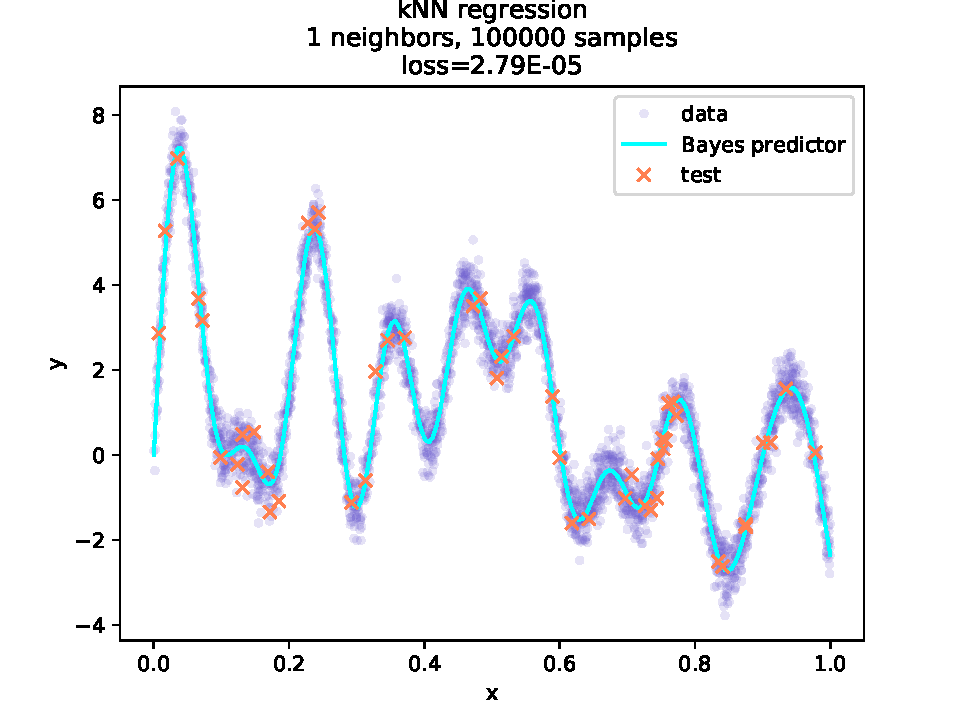
\includegraphics[width=0.9\linewidth]{knn}
    \label{fig:knn}
\end{figure}

\tableofcontents

\section*{\large\color{Blue}Presentation}

This document gathers important results and tools that will be used during the FTML course at Epita. It is not intended as an exhaustive course on the topic, as some results are stated without proof. It should rather be seen as a compact ressource of facts, definitions and results.

\section{\large\color{Blue}General mathematical results}

\subsection{\large\color{MidnightBlue}Linear algebra}

\subsubsection{\large\color{Periwinkle}Matricial writing of inner products}
\label{ssec:linalg}

In machine learning, optimization or statistics we often write the inner product of two vectors of $ \mathbb{R}^d$ as a product of matrices. If $x\in \mathbb{R}^d$ writes:
\begin{equation*}
x=\begin{pmatrix}
x_{1}\\
...\\
x_{i}\\
...\\
x_{d}
\end{pmatrix}
\end{equation*}

And (with $T$ denoting the transposition),
\begin{equation*}
y^T=\begin{pmatrix}
y_{1}, \dots y_j, \dots, y_d\\
\end{pmatrix}
\end{equation*}

Then we have that

\begin{equation*}
    \langle x, y \rangle = y^Tx=x^Ty
\end{equation*}

For instance, with this property we can show in a compact way that if $y\in \mathbb{R}^n$, $A\in \mathbb{R}^{n\times d}$, and $\theta\in \mathbb{R}^d$, then

\begin{equation*}
    \langle y, A\theta\rangle = \langle A^Ty, \theta\rangle
\end{equation*}

Indeed, 
\begin{equation*}
    \begin{aligned}
	\langle y, A\theta\rangle &= (A\theta)^Ty\\
	&= \theta^TA^Ty\\
	&=\theta^T(A^Ty)\\
	&=\langle \theta, A^Ty\rangle
    \end{aligned}
\end{equation*}

\subsection{\large\color{MidnightBlue}Statistics and Probability theory}

\subsubsection{\large\color{Periwinkle}Expected value, variance}

\begin{definition}{Moments of a distribution}

    Let $X$ be a real random variabe, and $k\in \mathbb{N}^*$. $X$ is said to have a moment of order $k$ if $E(|X|^k)<+\infty$, which means that:
    \begin{itemize}
	\item if $X$ is discrete, with image $X(\Omega)=(x_i)_{i\in \mathbb{N} }$, the series

	    \begin{equation*}
		\sum (x_i)^kP(X=x_i)
	    \end{equation*}

	    is \textbf{{absolutely}}  convergent. The moment is then equal to the sum of that series (without absolute value).
	\item is $X$ is continuous with density $p(x)$, the integral
	    \begin{equation*}
	        \int^{+\infty}_{-\infty} x^kf(x)  dx 
	    \end{equation*}
	    is \textbf{{absolutely}}  convergent. The moment is then equal to the sum of that series (without absolute value).
    \end{itemize}
\end{definition}

\begin{proposition}

    Let $k_1<k_2$ be integers. Let $X$ be a real random variable. Then if $X$ has a moment of order $k_2$, $X$ also has a moment of order $k_1$.
    
\end{proposition}

\begin{definition}{Expected value, variance}

    \begin{itemize}
        \item If $X$ has a moment of order $1$, it is called the \textbf{{expected value}} 
	\item If $X$ has a moment of order $2$, then $X-E(X)$ also has a moment of order $2$. This moment is called the variance of $X$.
	    \begin{equation*}
		V(X)=E\big((X-E(X))^2\big)
	    \end{equation*}
	    We often note $\sigma(X)= \sqrt{Var(X)}$. 
    \end{itemize}

\end{definition}

\begin{proposition}
    \label{prop:var}

    Let $a$ and $b$ be real numbers, and $X$ a random variable that admits a moment of order $2$. Then
    \begin{equation*}
	Var(aX+b)=a^2Var(X)
    \end{equation*}

\end{proposition}

\begin{proposition}
    Let $X$ and $Y$ be real two random variables that admit a moment of order $2$. Then the variable $XY$ has a moment of order $1$, and we then define the covariance of $X$ and $Y$ as
    \begin{equation*}
	Cov(X,Y) = E\big( (X-E(X))(Y-E(Y))\big)
    \end{equation*}
\end{proposition}
    

\begin{lemma}
    Let $X, Y, Z\in \mathbb{R} $ be real random variables with a moment of order $2$. We have:
\begin{equation*}
    Cov(X+Y, Z) = Cov(X,Z)+Cov(Y,Z)
\end{equation*}

\begin{equation*}
    Var(X+Y) = Var(X)+Var(Y)+2Cov(X,Y)
\end{equation*}

\begin{equation*}
    |Cov(X,Y)|\leq \sigma(X)\sigma(Y)
\end{equation*}
\end{lemma}

\begin{proposition}
    Let $(X_1, \dots, X_n)$ be $n$ mutually independent real random variables. Then if they all admit a moment of order $1$, then the product $X_1X_2\dots X_n$ also does admit a moment of order $1$ and 
    \begin{equation*}
	E(X_1X_2\dots X_n) = \prod^{n}_{i=1} E(X_i)
    \end{equation*}
    If they also admit moments of order $2$, then
    
    \begin{equation*}
	Var( \sum^{n}_{i=1} X_i ) = \sum^{n}_{i=1} Var(X_i)
    \end{equation*}
\end{proposition}

\begin{definition}{Expected value for vectors, variance matrix}

    From now on, if we write $E(X)$ or $Var(X)$, we implicitely assume that the quantities are correctly defined. Let $X\in \mathbb{R}^d$ be a random vector.
\begin{equation*}
X=\begin{pmatrix}
X_{1}\\
...\\
X_{i}\\
...\\
X_{d}
\end{pmatrix}
\end{equation*}

The \textbf{{expected value}} of the vector writes
\begin{equation*}
    E(X)=\begin{pmatrix}
    E[X_{1}]\\
...\\
    E[X_{i}]\\
...\\
    E[X_{d}]
\end{pmatrix}
\end{equation*}

    The \textbf{{variance matrix}} (or \textbf{{covariance matrix, variance-covariance, dispersion matrix}})  $Var(X)$ is defined as

    \begin{equation*}
	[Var(X)]_{ij} = Cov(X_i, X_j)       
    \end{equation*}
\end{definition}

\begin{lemma}
    If $A\in \mathbb{R}^{n,d}$, and $X = (X_1, \dots, X_d)^T$, $AX\in \mathbb{R}^n$, then we have

    \begin{equation*}
	E(AX)=AE(X)
    \end{equation*}
    and

    \begin{equation*}
	Var(AX) = AVar(X)A^T\in \mathbb{R}^{n, n}
    \end{equation*}
\end{lemma}

\begin{definition}{Independent and identically distributed variables}

    We say that the random variables $(X_n)_{n\in \mathbb{N} }$ are independent and identically distributed if $\forall i\in \mathbb{N} $, the law of $X_i$ is the same as the lax of $X_1$ and they are mutually independent. This is noted \textbf{{i.i.d variables.}} 
\end{definition}

\begin{remark}
    In machine learning, when studying a sequence of variables, each one representing for instance a sample drawn from a distribution, we most often assume that the resulting sequence is i.i.d.
\end{remark}


\subsubsection{\large\color{Periwinkle}Sample mean, sample variance, sample covariance}
\label{sec:empstats}

We observe a dataset $ \{x_i\in \mathbb{R}^d, i\in [1, n]\}$ of $n$ i.i.d samples. We assume that the underlying distribution has a moment of order $1$, noted $m\in \mathbb{R}^d$.

\begin{definition}{Sample mean vector}
    \begin{equation*}
	\bar{x} = \frac{1}{n} \sum^{n}_{i=1} x_i\in \mathbb{R}^d
    \end{equation*}
\end{definition}

\begin{remark}
The sample mean vector is an \textbf{{unbiased estimator}} of the expected value.

\begin{equation*}
    E( \bar{x}) = m
\end{equation*}
\end{remark}

\begin{definition}{Unbiased sample variance}

    If $d=1$, we define the \textbf{{unbiased sample variance}} by

    \begin{equation*}
	s^2= \frac{1}{n-1}  \sum^{n}_{i=1} (x_i- \bar{x})^2
    \end{equation*}
\end{definition}

\begin{remark}
    
    We assume that the underlying distribution has a moment of order $2$, noted $\sigma^2$. Then the unbiased sample variance is an \textbf{{unbiased estimator}} of the variance.

    \begin{equation*}
	E(s^2)=\sigma^2
    \end{equation*}

    If we replace the $ \frac{1}{n-1} $ factor by $ \frac{1}{n} $, we have a biased estimator. The use of $ \frac{1}{n-1} $ is called \textbf{{Bessel's correction}}. 
\end{remark}

\begin{definition}{Sample covariance matrix}

    We go back to the case of $ \{x_i\in \mathbb{R}^d, i\in [1, n]\}$. Each sample $x_i$ writes

\begin{equation*}
    x_i=\begin{pmatrix}
	x_{i1}\\
...\\
	x_{ij}\\
...\\
	x_{id}
\end{pmatrix}
\end{equation*}

    The sample covariance matrix is a $d\times d$ martix $S^2$ such that for all $(p,q)$

    \begin{equation*}
	S_{pq} = \frac{1}{n-1} \sum^{n}_{i=1} (x_{ip}- \bar{x}_p) (x_{iq}- \bar{x}_q) 
    \end{equation*}

    This can also be written

    \begin{equation*}
	S = \frac{1}{n-1} \sum^{n}_{i=1} (x_i- \bar{x})(x_i- \bar{x})^T
    \end{equation*}
\end{definition}

\begin{remark}
    The sample covariance matrix can also be written in a different way. We consider the \textbf{{sample matrix}} $X\in \mathbb{R}^{n,d}$.

    \begin{equation*}
    X=\begin{pmatrix}
	x_1^T\\
...\\
	x_i^T\\
...\\
	x_n^T
\end{pmatrix}
    \end{equation*}

    We can also consider the centered sample matrix defined by

    \begin{equation*}
	X_{\text{centered}}=\begin{pmatrix}
	x_1^T- \bar{x}^T\\
...\\
	x_i^T- \bar{x}^T\\
...\\
	x_n^T- \bar{x}^T
\end{pmatrix}
    \end{equation*}

    Then, the sample covariance matrix writes:

    \begin{equation*}
	S^2 = \frac{1}{n-1} X_{\text{centered}}^TX_{\text{centered}}
    \end{equation*}
\end{remark}

\subsubsection{\large\color{Periwinkle}Markov and Chebychev inequality}

\begin{proposition}{Markov inequality}

    Let $X$ ba a real non-negative random variable (variable aléatoire réelle positive), such that $E(|X|)<+\infty$. Let $a>0$. Then

    \begin{equation*}
	P(X\geq a)\leq \frac{E(X)}{a} 
    \end{equation*}
    
\end{proposition}

\begin{proposition}{Chebyshev inequality}
    Let $X$ ba a real random variable, such that $E(|X|^2)<+\infty$. Let $a>0$. Then

    \begin{equation*}
	P(|X-E[X]|>a)\leq \frac{Var(X)}{a^2} 
    \end{equation*}
\end{proposition}


\begin{theorem}{Weak law of large numbers}

    Let $(X_n)_{n\in \mathbb{N} }$ be a sequence of i.i.d. variables that have a moment of order $2$. We note $m$ their expected value. Then

    \begin{equation*}
	\forall \epsilon > 0, \lim_{n\rightarrow+\infty}P\big( |\frac{1}{n} \sum^{n}_{i=1} X_i-m|\geq \epsilon \big)= 0
    \end{equation*}

We say that we have \textbf{{convergence in probability}}.
\end{theorem}

\begin{proof}

    Let $S_n= \frac{1}{n} \sum^{n}_{i=1} X_i$. By linearity of the expected value, $E(S_n)=m$. We note $\sigma^2=Var(X_1)$. By independence of the sequence $(X_n)_{n\in \mathbb{N} }$, we have that $Var(S_n)= \sum^{n}_{i=1} Var( \frac{1}{n}  X_i)$, which is equal to $ \frac{1}{n^2} \sum^{n}_{i=1} Var(X_i)= \frac{\sigma^2}{n} $ with \ref{prop:var}.

    Using the Chebychev inequality, 

    \begin{equation*}
        \begin{aligned}
	    P(|S_n-m|>\epsilon) &\leq \frac{Var(S_n)}{\epsilon^2} \\
	    &= \frac{\sigma^2}{n\epsilon^2} 
        \end{aligned}
    \end{equation*}
    
\end{proof}

\begin{remark}
    Keeping the same hypotheses on the sequence of variables, we can make some important observations.
    \begin{itemize}
	\item $\lim_{n\rightarrow +\infty}Var(S_n)=0$.
	\item More precisely, we have a probabilistic bound on the magnitude of the difference between the average $S_n$ and $m$.

	    \begin{equation*}
		\sqrt{Var\Big( S_n-m \Big)} = \frac{\sigma}{ \sqrt{n} } 
	    \end{equation*}
    \end{itemize}
\end{remark}


\subsubsection{\large\color{Periwinkle}Concentration inequalities}

Concentration inequalities are useful in order to have \textbf{{non-asymptotic }} bounds on the deviation between the average of random variables and their mean. Non-asymptotic means that we have an inequality for all $n$, as opposed to the central limit theorem that is asymptotic and holds for $n\rightarrow+\infty$.

\begin{theorem}{Bernstein inequality}
Let $u_1, \dots, u_n$ be i.i.d. random variables, such that $E(u)=0$ and $|u|\leq B$ almost surely, with $B>0$. Let $ \sigma^2=E(u^2)$ and $t>0$:

\begin{equation*}
    P( \frac{1}{n} \sum^{n}_{i=1} u_i >t)\leq e^{ - \frac{t^2n/2}{\sigma^2+bt} }
\end{equation*}
\end{theorem}

\begin{corollary}
    Under the same assumptions:
\begin{equation*}
    P( |\frac{1}{n} \sum^{n}_{i=1} u_i |>t)\leq 2e^{ - \frac{t^2n/2}{\sigma^2+bt} }
\end{equation*}
    
\end{corollary}

\begin{theorem}{Hoeffding's inequality}

    Let $(X_i)_{1\leq i\leq n}$ be $n$ i.i.d real random variables such that $\forall i\in [1, n]$, $X_i\in [a,b]$ and $ E(X_i)= \mu \in \mathbb{R} $.  Let $	\bar{\mu} = \frac{1}{n} \sum^{n}_{i=1} X_i$.

    Then $\forall \epsilon >0$,

    \begin{equation*}
	P\Big(| \bar{\mu}-\mu|\geq \epsilon \Big) \leq 2 \exp\Big( -\frac{2n\epsilon^2}{(b-a)^2} \Big)
    \end{equation*}
\end{theorem}

\subsection{\large\color{MidnightBlue}Differential calculus}

\subsubsection{\large\color{Periwinkle}Differentiable functions}

\begin{definition}{Differentiable function}
    \label{def:diff}

    Let $V$ and $W$ be real Hilbert spaces (complete vector space with an inner product). Let $f: V\rightarrow W $. We say that $f$ is differentiable in $x\in V$ if there exsists a continuous linear application $L_x:V\rightarrow \mathbb{R} $ such that

    \begin{equation*}
	f(x+h)=f(x)+L_x(h)+o(h)
    \end{equation*}

    with $ \lim_{h\rightarrow 0} \frac{|o(h)|}{||h||} =0$.
\end{definition}

\begin{remark}

    We consider the case (that we will often encounter) where $W= \mathbb{R}$. Then for a fiven $x\in B$, $L_x$ is a linear form, and since $V$ is a Hilbert space, with Riesz representation theorem we know that, there exists a unique vector $p_x\in V$ such that $\forall h\in V, L_x(h)= \langle p, h \rangle$. $p$ is sometimes noted $f'(x)$,  $ \nabla_xf$ or $\nabla f(x)$. We note that we do not assume here that $V$ is of finite dimension.
    
\end{remark}

\begin{definition}{Two times differentiable function}

    We keep the same hypotheses as in \ref{def:diff} and assume that $W= \mathbb{R}$. If the application $x\mapsto \nabla_xf $ is differentiable in $x$, the we say that $f$ is two times differentiable in $x$. In that case we note $f"(x)$ the second-order derivative, that satisfies:

    \begin{equation*}
	\nabla_{x+h}f=\nabla_xf+f"(x)(h)+o(h)
    \end{equation*}
\end{definition}

\begin{lemma}
    We keep the same hypotheses. Given $x$ and $h$, $f"(x)(h)$ is an element of $V$, that can also be identified to an element of its dual space $V^*$. With the notation $f"(x)(h, h')=f"(x)(h)(h')$, we can show that

    \begin{equation*}
	f(x+h)=f(x)+\nabla_xf(h)+ \frac{1}{2} f"(x)(h,h)+o(||h||^2)        
    \end{equation*}
\end{lemma}

\subsubsection{\large\color{Periwinkle}Jacobian matrix, gradient and Hessian}

In this paragraph, we consider the case when $V= \mathbb{R}^d$, which is the most frequent situation encountered in machine learning.
\\

\textbf{{Jacobian matrix:}} If $f: \mathbb{R}^d\rightarrow \mathbb{R}^p$ is differentiable on $ \mathbb{R}^d$ we note $L^f_x$ the differential in $x$. It is an application from $ \mathbb{R}^d$ to $ \mathbb{R}^p$. We can then equivalently consider its matrix, that can be noted also $L^f_x\in \mathbb{R}^{p, d}$. 

\begin{equation*}
    f(x+h)=f(x)+L^f_xh+o(h)
\end{equation*}

$L^f_x$ is called the \textbf{{Jacobian matrix}}  of $f$ in $x$.
\\

\textbf{{Link with the gradient}}: we note that if the function $f$ has real values ($p=1$), then 

\begin{equation*}
    \nabla_xf=(L^f_x)^T\in \mathbb{R}^{d, 1}
\end{equation*}

\textbf{{Jacobian of a product.}} 

If we now consider $g: \mathbb{R}^p\rightarrow \mathbb{R}^q$ another differentiable application, and note its matrix / differential in $f(x)$ as $L^g_{f(x)}\in \mathbb{R}^{q, p}$, we have:

\begin{equation*}
    \begin{aligned}
	(g\circ f)(x+h)&=g(f(x+h))\\
	&=g(f(x)+L^f_xh+o(h))\\
	&=g(f(x)+L^f_xh)+L^g_{f(x)}o(h)+o(o(h))\\
    \end{aligned}
\end{equation*}

We can show that $L^g_{f(x)}o(h)+o(o(h))=o(h)$. Hence, 

\begin{equation*}
    \begin{aligned}
	(g\circ f)(x+h)&=g(f(x)+L^f_xh)+o(h)\\
	&=g(f(x))+L^g_{f(x)}L^f_xh+o(L^f_xh)+o(h)\\
    \end{aligned}
\end{equation*}

We can also show that $o(L^f_xh)=o(h)$, for instance using the operator norm of $L^f_x$.

Finally, the Jacobian matrix $L^{g\circ f}_x$ of $g\circ f: \mathbb{R}^d\rightarrow \mathbb{R}^q$ in $x$ is the product of the jacobians.

\begin{equation}
    \label{eq:jacobprod}
    L^{g\circ f}_x=L^{g}_{f(x)}L^f_x\in \mathbb{R}^{q, d}
\end{equation}


\textbf{{Gradient of a product:}} 
With the same functions $g$ and $f$ and if $q=1$, we deduce from \ref{eq:jacobprod} that 

\begin{equation*}
    \begin{aligned}
	\nabla_x(g\circ f)&= (L^{g\circ f}_x)^T\\
	&=(L^{g}_{f(x)}L^f_x)^T\\
	&=(L^f_x)^T(L^{g}_{f(x)})^T\\
	&= (L^f_x)^T\nabla_{f(x)}g\in \mathbb{R}^{d, 1}
    \end{aligned}
\end{equation*}

\textbf{{Hessian}}: if $f: \mathbb{R}^d\rightarrow \mathbb{R} $ is two times differentiable in $x$, then the application $\nabla f: \mathbb{R}^d\rightarrow \mathbb{R}^d$, $x\mapsto\nabla_xf$ has a matrix $H^f_x\in \mathbb{R}^{d,d}$, called the Hessian.

\begin{equation*}
    \nabla_{x+h}f=\nabla_xf+H^f_xh+o(h)
\end{equation*}

Then, the development of $f$ around $x$ can be written

\begin{equation*}
    f(x+h)=f(x)+L^f_xh+ \frac{1}{2} h^T(H^f_x)h+o(||h||^2)
\end{equation*}

\textbf{{Examples}} 

\begin{itemize}
    \item[ \textbf{{Quadratic function}}] Let $A\in \mathbb{R}^{d,d}$ be a symmetric real matrix. If $f(x)= \frac{1}{2} x^TAx-b^Tx$, then
	\begin{itemize}
	    \item $\nabla_xf=Ax-b$ 
	    \item $H_x^f=A$.
	\end{itemize}
    \item[ \textbf{{Least squares}} ] Let $X\in \mathbb{R}^{n,d}$, $\theta\in \mathbb{R}^d$, $y\in \mathbb{R}^n$. If $f(\theta)= \frac{1}{2} ||X\theta-y||_2^2$, then
	\begin{itemize}
	    \item $\nabla_{\theta}f=X^T(X\theta-y)$
	    \item $H_{\theta}^f=X^TX$.
	\end{itemize}
\end{itemize}

\textbf{{Explicit formulation of the gradient, the Jacobian, the Hessian}}. We assume $f: \mathbb{R}^d\rightarrow  \mathbb{R}^p $ is differentiable.

\begin{equation*}
    \forall x\in \mathbb{R}^d, f(x)=
\begin{pmatrix}
    f_1(x)\\
...\\
    f_{i}(x)\\
...\\
    f_{d}(x)
\end{pmatrix}
\end{equation*}

\begin{equation*}
L^f_x=
\begin{pmatrix}
    \frac{\partial f_1}{\partial x_1}(x)  & \frac{\partial f_1}{\partial x_2}(x) & \dots & \frac{\partial f_1}{\partial x_d}(x) \\
\dots & \dots & \dots & \dots \\
\dots & \dots & \dots & \dots \\
    \frac{\partial f_p}{\partial x_1}(x)  & \frac{\partial f_p}{\partial x_2}(x) & \dots & \frac{\partial f_p}{\partial x_d}(x) \\
\end{pmatrix}
\end{equation*}

If $f$ has real values ($p=1$), then
\begin{equation*}
    \nabla_xf=
    \begin{pmatrix}
	\frac{\partial f}{\partial x_1} (x)\\
...\\
	\frac{\partial f}{\partial x_i}(x) \\
...\\
	\frac{\partial f}{\partial x_d} (x)\\
\end{pmatrix}
\end{equation*}

and if we keep $p=1$ and assume that $f$ is two times differentiable, then the Hessian reads:

\begin{equation*}
H^f_x=
\begin{pmatrix}
    \frac{\partial^2 f}{\partial^2 x_1}(x)  & \frac{\partial^2 f}{\partial x_2\partial x_1}(x) & \dots & \frac{\partial^2 f}{\partial x_d\partial x_1}(x) \\
\dots & \dots & \dots & \dots \\
\dots & \dots & \dots & \dots \\
    \frac{\partial^2 f}{\partial x_1\partial x_d}(x)  & \frac{\partial^2 f}{\partial x_2\partial x_d}(x) & \dots & \frac{\partial^2 f}{\partial x_d^2}(x) \\
\end{pmatrix}
\end{equation*}

\begin{remark}
    By Swhartz theorem, if $f$ is $C^2$, then the Hessian is symmetrical.
\end{remark}




\subsubsection{\large\color{Periwinkle}Lipshitz continuity}
\label{def:lipshitz}

\begin{definition}{L-Lipschitz continuous function}

    Let $f$ be a differentiable function and $L>0$. We say that $f$ is $L$-Lipschitz continuous if $\forall x,y\in \mathbb{R}^d$, 
    \begin{equation*}
	||f(x)-f(y)||\leq L||x-y||
    \end{equation*}
\end{definition}

\begin{definition}{L-Lipschitz continuous gradients}

    Let $f$ be a differentiable function and $L>0$. We say that $f$ has $L$-Lipschitz continuous gradients if $\forall x,y\in \mathbb{R}^d$, 
    \begin{equation*}
	||\nabla_xf-\nabla_yf||\leq L||x-y||
    \end{equation*}
\end{definition}


\subsubsection{\large\color{Periwinkle}Smoothness}

\begin{definition}{Smoothness}

    A differentiable function $f$ with real values is said $L$-smooth if and only if
    \begin{equation*}
	\forall x, y\in \mathbb{R}^d, |f(y)-f(x)-\nabla_xf(y-x)|\leq \frac{L}{2} ||y-x||^2
    \end{equation*}
\end{definition}

\begin{lemma}
    $f$ is $L$-smooth if and only if it has $L$-Lipshitz continuous gradients.
\end{lemma}

\begin{lemma}
    
    If $f$ is twice differentiable, $f$ is $L$-smooth if and only if
    \begin{equation*}
        \forall x\in \mathbb{R}^d, -LI_d\leq H_xf\leq LI_d
    \end{equation*}

	 Meaning that all eigenvalues of $H_xf$ have a module that is smaller than $L$. Here, $\geq$ denotes the \textbf{{Loewner order}}, which is a partial order on symmetric matrices. \url{https://en.wikipedia.org/wiki/Loewner_order}.
\end{lemma}

\subsection{\large\color{MidnightBlue}Algorithmic complexities}

In machine learning, there is a focus on the efficiency of algorithm, as large-scale problems are frequent and some algorithmic complexities are prohibitive. We give some reminders on orders of magnitudes of time-complexity of some operations, ignoring space complexity in this section.

\begin{itemize}
    \item If $A\in \mathbb{R}^{d, d}$ is invertible, the cost of inverting it is $ \mathcal{O} (d^3)$.
    \item If $A\in \mathbb{R}^{d, d}$ is symmetric, the cost of computing its eigenvalues and eigenvectors $ \mathcal{O} (d^3)$.
    \item If $X\in \mathbb{R}^{n,d}$ and $\theta\in \mathbb{R}^d$, the cost of computing $ X\theta\in \mathbb{R}^n$ is $ \mathcal{O} (nd)$.
\end{itemize}

Some optimisations of these operations exist, see:
\begin{itemize}
    \item QR decomposition for matrix inversion (\url{https://en.wikipedia.org/wiki/QR_decomposition}).
    \item Low-rank approximation. \url{https://en.wikipedia.org/wiki/Low-rank_approximation} 
\end{itemize}

\section{\large\color{Blue}Optimization}

Reference: \cite[]{Allaire2012} 

\subsection{\large\color{MidnightBlue}Definitions}

\begin{definition}{Minima}
    Let $f: \mathbb{R}^d\rightarrow \mathbb{R}$ be defined on $K\subset \mathbb{R}^d$.

    $x\in K$ is a local minimum of $f$ on $K$ if and only if
    \begin{equation*}
	\exists \delta>0, \forall y\in K, ||y-x||<\delta \Rightarrow f(x)\leq f(y)
    \end{equation*}

    $x\in K$ is a global minimum of $f$ on $K$ if and only if
    \begin{equation*}
	\forall y\in K, f(x)\leq f(y)
    \end{equation*}
\end{definition}

\begin{definition}{Coercive function}

    $f:V\rightarrow \mathbb{R} $, defined on a vector space, $V$ is \textbf{{coercive}} if 
    \begin{equation*}
	\lim_{||x||\rightarrow +\infty}f(x)=+\infty
    \end{equation*}
\end{definition}

\subsection{\large\color{MidnightBlue}Existence result}

\begin{theorem}{Existence of a global minimum in $\mathbb{R}^d$}

    Let $K$ be a closed non-empty subset of $ \mathbb{R}^d$, and $f: \mathbb{R}^d\rightarrow \mathbb{R} $ a continuous coercive function. Then, there exists at least a global minimum of $f$ on $K$.
\end{theorem}

\subsection{\large\color{MidnightBlue}Convex analysis}

Convexity is a key property of function, that allows to have theoretical proofs on the existence of solutions to a optimization problem, and on the convergence of optimization algorithms. It is useful in finite dimensional spaces and also in infinite dimensional spaces.

\subsubsection{\large\color{Periwinkle}Definitions}

\begin{definition}{Convex function}

    The function $f:\Omega \rightarrow \mathbb{R} $ with $\Omega$ convex is:
    \begin{itemize}
	\item \textbf{{convex}} if $\forall x, y\in \Omega, \alpha\in [0,1]$,
	    \begin{equation*}
		f(\alpha x+(1-\alpha)y)\leq \alpha f(x)+(1-\alpha)f(y)
	    \end{equation*}
	\item \textbf{{strictly convex}} if $\forall x, y\in \Omega, \alpha\in [0,1]$,
	    \begin{equation*}
		f(\alpha x+(1-\alpha)y)< \alpha f(x)+(1-\alpha)f(y)
	    \end{equation*}
	\item $\mu$-\textbf{{strongly convex}} if $\forall x, y\in \Omega, \alpha\in [0,1]$,
	    \begin{equation*}
		f(\alpha x+(1-\alpha)y)\leq \alpha f(x)+(1-\alpha)f(y)- \frac{\mu}{2} \alpha(1-\alpha)||x-y||^2
	    \end{equation*}
    \end{itemize}
\end{definition}

\begin{lemma} Let $f$ be convex on convex set $ \Omega$, $f:\Omega \rightarrow \mathbb{R} $.  Let $c\in \mathbb{R} $. Then

\begin{equation*}
    \Omega_c = \{x\in \Omega, f(x)\leq c\}
\end{equation*}
 
 is a convex set.
\end{lemma}

\begin{proposition}
    $f$ is $ \mu$ convex if and only if $ x\mapsto f(x)- \frac{\mu}{2} ||x||^2$ is convex.
\end{proposition}

\textbf{{Examples:}} 

\begin{itemize}
    \item All norms are convex.
    \item $x\mapsto \log(1+e^{-x})$ is convex on $ \mathbb{R} $
    \item $x\mapsto \theta^Tx$ is convex on $ \mathbb{R}^d$ with $\theta \in \mathbb{R}^d$ (linear form)
    \item if $Q$ is a symmetric semidefinite positive matrix (matrice positive), then the positive quadratic form $x\mapsto x^TQx$ is convex.
    \item if $Q$ is a symmetric definite positive matrix (matrice définie positive) with smallest eigenvalue $\lambda_{min}>0$, then the positive definite quadratic form $x\mapsto x^TQx$ is $ 2\lambda_{min}$- strongly convex.
    \item if $X\in \mathbb{R}^{n\times d}$, and $Y\in \mathbb{R}^n$, $\theta\mapsto ||X\theta-Y||^2$ is convex on $ \mathbb{R}^d$ (Least-squares)
    \item If $f$ is increasing and convex and $g$ is convex, then $f \circ g $ is convex.
    \item Is $f$ in convex and $g$ is linear, then $f \circ g $ is convex.
\end{itemize}

\begin{definition}{Condition number}

    If $f$ is $L$-smooth and $\mu$-strongly convex, we define its \textbf{{condition number}} as:

    \begin{equation*}
        \kappa = \frac{L}{\mu} 
    \end{equation*}

\end{definition}

\begin{remark}
    The condition number is an important quantity to consider when studying the convergence speed of gradient algorithms.
\end{remark}


\subsubsection{\large\color{Periwinkle}Differential formulation of convexity}

\begin{proposition}
    \label{prop:conv}
    Let $f:V \rightarrow \mathbb{R} $ be a differentiable function. The following conditions are equivalent.
    \begin{itemize}
        \item $f$ is convex.
	\item $\forall x, y\in V, f(y)\geq f(x)+(f'(x)|y-x)$ ($f$ is above its tangent space)
	\item $\forall x, y\in V, (f'(x)-f'(y)|x-y)\geq 0$ ($f'$ grows)
    \end{itemize}
\end{proposition}

\begin{remark}
    Equivalently
    \begin{equation*}
	\forall u,v\in V, f(u)-f(v)\leq f'(u)(v-u)
    \end{equation*}
\end{remark}

\begin{proposition}
    \label{prop:alphaconv}
    Let $f:V \rightarrow \mathbb{R} $ be a differentiable function, and $\mu>0$. The following conditions are equivalent.
    \begin{itemize}
        \item $f$ is $ \mu$-convex
	\item $\forall x, y\in V, f(y)\geq f(x)+(f'(x)|y-x)+ \frac{  \mu}{2} ||y-x||^2$
	\item $\forall x, y\in V, (f'(x)-f'(y)|x-y)\geq \mu ||x-y||^2$
    \end{itemize}
\end{proposition}

\begin{lemma}{Lojasiewicz inequality}

    Let $f: \mathbb{R}^d\rightarrow \mathbb{R} $ be a $\mu$-strongly convex differentiable function with a unique minimiser $x^*$. Then, we have that for all $x\in \mathbb{R}^d$, 

    \begin{equation*}
	||\nabla_xf||_2^2\geq 2\mu \big(f(x)-f(x^*)\big)
    \end{equation*}
\end{lemma}

\begin{proposition}{Convexity of two-times differentiable functions}

    We now assume that $f$ is two times differentiable.

    \begin{itemize}
	\item $f$ is convex if anf only if
	    \begin{equation*}
		\forall x, h\in y, J"(x)(h, h)\geq 0
	    \end{equation*}
	\item $f$ is $\mu$-strongly convex if and only if
	    \begin{equation*}
		\forall x, h\in y, J"(x)(h, h)\geq \mu ||h||^2
	    \end{equation*}
    \end{itemize}

\end{proposition}

\begin{remark}
    In the case of $V= \mathbb{R}^d$, the two previous conditions mean respectively that 

	    \begin{equation}
		\label{eq:hessconv}
		\forall x, h\in y, h^T(H_xf)h\geq 0
	    \end{equation}

	    and

	    \begin{equation}
		\label{eq:hessconvmu}
		\forall x, h\in y, h^T(H_xf)h\geq \mu ||h||^2
	    \end{equation}

	    \ref{eq:hessconv} means that $\forall x\in \mathbb{R}^d$, all eigenvalues of $H_xf$ are non-negative, while \ref{eq:hessconvmu} means that they all are $\geq \mu$.



\end{remark}

\subsubsection{\large\color{Periwinkle}Minima of convex functions}

\begin{proposition}
    \label{prop:miniconv}

    \begin{itemize}
        \item If $f$ is convex, any local minimum is a global minimum. The set of global minimizers is a convex set.
	\item If $f$ is strictly convex, there exists at most one local minimum (that is thus global).
	\item If $f$ is convex and $C^1$ (differentiable, $a\mapsto df_a$ continuous), then $x$ is a minimum (thus global) of $f$ on $V$ if and only if the gradient cancels in $x$, $\nabla_xf=0$. $V$ need not be finite-dimensional.
    \end{itemize}
\end{proposition}

\subsubsection{\large\color{Periwinkle}Existence of a global minima for convex functions}

\begin{theorem}{Existence of a global minimum, strongly convex case}
    \label{th:alphaconv}

    Let $K$ be a closed non-empty subset of the Hilbert space $H$, and $f: \mathbb{R}^d\rightarrow \mathbb{R} $ a continuous $\mu$-strongly convex function. Then, there exists a unique a global minimum $u$ of $f$ on $K$, and

    \begin{equation*}
	\forall y\in K, ||y-x||^2\leq \frac{ \alpha}{4} [ f(y)-f(x)]
    \end{equation*}
\end{theorem}

\begin{theorem}{Existence of a global minimum, convex case}
    \label{th:alphaconv}

    Let $K$ be a closed non-empty subset of the Hilbert space $H$, and $f: \mathbb{R}^d\rightarrow \mathbb{R} $ a continuous convex coercive function. Then, there exists a global minimum $u$ of $f$ on $K$.

\end{theorem}

\subsubsection{\large\color{Periwinkle}Local minimum of a two-times differentiable function}

\begin{theorem}
    
We assume that $K=V$ ans $f$ is two-times différentiable in $x$.

If $x$ is a local minimizer of $f$, then
\begin{itemize}
    \item $f'(x)=0$
    \item $\forall h\in V, f"(u)(h,h)\geq 0$
\end{itemize}


\end{theorem}

\begin{remark}
    
    In this theorem, we do not assume that $f$ is convex.
\end{remark}

\begin{remark}
   When  $V= \mathbb{R}^d$, the previous conditions translate in the fact that $H_xf$ is positive semi-deminite or that $H_yf$ is positive semidefinite in a neighborhood of $x$. 
\end{remark}


\subsubsection{\large\color{Periwinkle}Expected values and convex functions}

Let $D$ be a convex set. If $f$ is convex, then if $p: S\Rightarrow D$ is such that $p(x)\geq 0$ and $ \int_{S} p(x)  dx =1$, then

\begin{equation*}
    f( \int_{S} p(x)x  dx)\leq \int_{S} p(x)f(x)  dx
\end{equation*}

Let $D$ be a convex set. If $X$ is a random variable such that $ X\in D$ almost surely and $ E[X]$ exists, then

\begin{equation*}
    f(E[X])\leq E[f(X)]
\end{equation*}

\subsection{\large\color{MidnightBlue}Gradient Descent (GD)}

\subsubsection{\large\color{Periwinkle}Context}

GD is an important first-order algorithm for optimization. First-order means that it is based on the first-order derivative. For well-conditioned convex problems, it converges exponentially fast. We want to minimize a differentiable function $f$. The \textbf{{gradient descent (GD)}}  update reads:

\begin{equation*}
    x_{t+1} = x_t - \gamma_t \nabla f(x_t)
\end{equation*}

\subsubsection{\large\color{Periwinkle}Minimisation of a strongly convex function}

The following lemma shows that if the step size is small enough, then GD is a \textbf{{descent algorithm.}} 

\begin{lemma}
    let $L>0$, $f: \mathbb{R}^d\rightarrow \mathbb{r} $ a convex function with $L$-lipshitz continuous gradients (see \ref{def:lipshitz}). Let $x_0\in \mathbb{R}^d$, $\gamma_t >0$. Then

    \begin{equation*}
	f(x_t)\leq f(x_{t-1})-\gamma_t (1-L\gamma_t) ||\nabla f(x_{t-1})||^2
    \end{equation*}

    In particular if $0<  \gamma_t < \frac{1}{L} $, then $ \forall t\in \mathbb{N} $ such that $ x_{t-1}$ is not a global minimum,

    \begin{equation*}
	f(x_t)<f(x_{t-1})
    \end{equation*}

    Otherwise $x_t = x_{t-1}$ and $f(x_t) = f(x_{t-1})$.
\end{lemma}

\begin{theorem}{Convergence of GD for a strongly convex function}

    Let $f: \mathbb{R}^d\Rightarrow \mathbb{R}	$ be a  $\mu$-strongly convex unction with $L$-Lipshitz continuous gradients. Let $x^*$ be the global minimum of $f$ (which we know exists since $f$ is strongly convex), $x_0\in \mathbb{R} $, $T\in \mathbb{N}$.

    \begin{itemize}
	\item With constant step size $\gamma_t = \frac{1}{L} $, we have

	    \begin{equation*}
		f(x_t)-f(x^*)\leq ( 1- \frac{\mu}{L})^t\big(f(x_0)-f(x^*)\big) 
	    \end{equation*}
        \item With constant step size $0<\gamma < \frac{1}{2l} $, we have

    \begin{equation}
	\label{eq:gdconv}
	||x_t-x^*||^2\leq (1-\gamma \mu)^T ||x_0-x^*||^2
    \end{equation}
    \end{itemize}
\end{theorem}

\begin{remark}
    \ref{eq:gdconv} could seem surprising at first sight, since it implies that $ (1-\mu\gamma)\geq 0$ if $0<\gamma< \frac{1}{2l}$. However, we have
\begin{equation*}
    \mu ||x-y||^2\leq \langle \nabla_xf-\nabla_yf, x-y \rangle \leq L||x-y||^2
\end{equation*}

Hence, $\mu\leq L$, so $\mu\gamma < \frac{1}{2} $.
\end{remark}

\begin{corollary}
    We note that $ (1-\gamma \mu)^T = (1- \frac{ \gamma \mu T}{T} )^T\leq e^{-\gamma \mu T}$. Thus,

    \begin{equation*}
	||x_t-t^*||^2\leq e^{-\gamma\mu T}||x_0-x^*||^2
    \end{equation*}

    We call this an \textbf{{exponential convergence}}. It is also sometimes called \textbf{{linear convergence}}. We can deduce that if 
    \begin{equation*}
	T \geq \frac{1}{ \gamma \mu} \log \big( \frac{||x_0-x^*||^2}{\epsilon}  \big)
    \end{equation*}
    then

    \begin{equation*}
        ||x_T-x^*||\leq \epsilon
    \end{equation*}
\end{corollary}

\subsubsection{\large\color{Periwinkle}Minimization of a convex function}

\begin{theorem}{Convergence of GD for a smooth convex function}

    Let $f: \mathbb{R}^d\rightarrow \mathbb{R} $, with global minimiser $x^*$. With constant step-size $\gamma_t = \frac{1}{L} $, the iterates $x_t$ of GD satisfie:

    \begin{equation*}
	f(x_t)-f(\eta^*)\leq \frac{L}{2t} ||x_0-\eta^*||^2
    \end{equation*}
\end{theorem}


\section{\large\color{Blue}Supervised Learning}

\subsection{\large\color{MidnightBlue}General definitions and bounds}

\subsubsection{\large\color{Periwinkle}Setup}

Given some \textbf{{observations}} $(x_i,y_i)\in \mathcal{X} \times \mathcal{Y}$ of input/output pairs, we would like to predict well the new output $y\in \mathcal{Y} $ that should be associated with a new input $x\in \mathcal{X} $. The training dataset is noted $D_n = \{(x_i, y_i), i\in [1, \dots, n]\}$.

We assume that there exists an \textbf{{unknown distribution}} $\rho$ for the joint variable $(X,Y)$.  In most theoretical frameworks used to study Supervised Learning, each sample $(x_i,y_i)$ is assumed to be drawn independently from this law. Hence, $D_n$ is a \textbf{{random variable.}} 

\begin{equation*}
    (x_i,y_i)\sim \rho, \forall i\in[1, n]
\end{equation*}

A \textbf{{learning rule}} $ \mathcal{A} $ is a application that associates a \textbf{{prediction function}}, or \textbf{{estimator}}  $ \tilde{f}_n$, to $D_n$.

$$
\mathcal{A}  : \left\{
    \begin{array}{ll}
	\cup_{n\in \mathbb{N} } ( \mathcal{X} \times \mathcal{Y} )^n\rightarrow \mathcal{Y}^{ \mathcal{X} } & \\
        D_n \mapsto \tilde{f}_n& 
    \end{array}
\right.
$$

Since $D_n$ is a random variable, and since $ \tilde{f}_n$ depends on $D_n$, $ \tilde{f}_n$ is also a random variable.

\subsubsection{\large\color{Periwinkle}Definitions}

\begin{definition}{Loss}

    A \textbf{{loss}} $l$ is an application that measures the discrepancy between to elements of a set (for instance of a linear space).
$$
l: \left\{
    \begin{array}{ll}
	\mathcal{Y} \times \mathcal{Y} \rightarrow \mathbb{R}_+ & \\
	(y,y') \mapsto l(y,y')& 
    \end{array}
\right.
$$

\end{definition}

\begin{definition}{Risks}

    Let $l$ be a loss.

    The \textbf{{risk}} (or \textbf{{statistical risk, generalization error, test error)}} of estimator $f$ writes

    \begin{equation*}
	E_{(X,Y)\sim \rho}[l(Y,f(X)]
    \end{equation*}

    The \textbf{{empirical risk (ER)}} of an estimator $f$ writes

    \begin{equation*}
	R_n(f) = \frac{1}{n} \sum^{n}_{i=1} l(y_i, f(x_i))
    \end{equation*}

    We emphasize that the risks depends on the loss $l$.
\end{definition}

\begin{remark}

    \begin{equation*}
	R_n(f)=E_{(X,Y)\sim \rho_n}[l(Y,f(X)]
    \end{equation*}
\end{remark}

We define the \textbf{{target function}} $f^*$ by

\begin{equation*}
    f^*\in \argmin_{f:X\rightarrow Y} R(f)
\end{equation*}

with $f:X\rightarrow Y$ set of measurable functions.


\begin{definition}{Fundamental problem of Supervised Learning}

    Estimate $f^*$ given only $D_n$ and $l$.
    
\end{definition}

\begin{definition}{Excess risk}

    The \textbf{{excess risk}} $ \mathcal{R} ( \tilde{f}_n)$ measures how close  $ \tilde{f}_n$ (predictor obtained by ERM) is to the best possible $f^*$, in terms of expected risk (average / expecter) error on new examples.

    \begin{equation*}
	\mathcal{R} ( \tilde{f}_n) = R( \tilde{f}_n)-R(f^*)
    \end{equation*}

    We also define the \textbf{{excess probability}} as
    \begin{equation*}
	P\big( R( \tilde{f}_n)-R(f^*)>t\big), \forall t>0
    \end{equation*}
\end{definition}

\begin{remark}
Since $ \tilde{f}_n$ is a random variable $D_n$, $R_n( \tilde{f})$ and thus $ \mathcal{R} ( \tilde{f}_n)$ are also random variables.
\end{remark}


\begin{definition}{Consistency}

    The algorithm $\mathcal{A} $ is said to be \textbf{{consistent}}  if 

    \begin{equation*}
	\lim_{n\rightarrow +\infty} E_{D_n} \mathcal{R} ( \tilde{f}_n)=0 
    \end{equation*}
\end{definition}

    We also say that $ \mathcal{A} $ is a \textbf{{learning algorithm.}} 

\begin{definition}{Strong consistency}

    The algorithm $\mathcal{A} $ is said to be \textbf{{strongly consistent}}  if with probability $1$

    \begin{equation*}
	\lim_{n\rightarrow +\infty} \mathcal{R} ( \tilde{f}_n)=0 
    \end{equation*}


\end{definition}

\begin{definition}{Learning Rates}

    The sequence $(e_n)_{n \in \mathbb{R} } $ is a learning rate in expectation if

    \begin{equation*}
	E_{D_n} [\mathcal{R} ( \tilde{f}_n)]\leq e_n, \forall n\in \mathbb{N} 
    \end{equation*}
    
\end{definition}

\begin{definition}{Learning rate in probability}

    Let $\delta \in ]0, 1]$.  The  sequence $(p_{n, \delta})_{n\in \mathbb{N} }$ is a learning rate in probability if

    \begin{equation*}
	P_{D_n}( \mathcal{R} ( \tilde{f}_n)\geq p_{n,\delta})\leq \delta, \forall n\in \mathbb{N} 
    \end{equation*}
\end{definition}


    \subsubsection{\large\color{Periwinkle}Bayes predictor and conditional expectation}

    Under some conditions, we can give an explicit formulation of $f^*$, the best predictor in $ \mathcal{Y}^{ \mathcal{X} }$, although we can not compute it without the knowledge of the distribution of $(X,Y)$. In this paragraph we ignore the measurability issues that were mentioned earlier.

    \begin{theorem}{Bayes predictor}
        
	If $ \mathcal{Y} $ is compact and $l$ is continuous, we have

	\begin{equation}
	    \label{eq:bayes}
	    f^*(x) = \argmin_{y\in \mathcal{Y} }E[ l(Y, y)|X=x]
	\end{equation}

	almost everywhere. $E[q(Y)|X=x]$ denotes the conditional expectation of $q(Y)$ given that $X=x$, with $ q:Y\mapsto \mathbb{R} $. $f^*$ is also called the \textbf{{Bayes}} predictor.
    \end{theorem}

    \begin{definition}{Bayes risk}

	The Bayes risk is the risk of the Bayes predictor.

	\begin{equation*}
	    R^* = E_X\Big( \inf_{y\in \mathcal{Y} }E\big( l(Y, y)|X\big) \Big)
	\end{equation*}
    \end{definition}


    \begin{remark}
	\begin{itemize}
	    \item $Y$ is a random variable while the parameter $y$ in \ref{eq:bayes} is a scalar.
	    \item As we do not know the joint distribution $\rho$, it is not possible to compute the Bayes predictor from this expression.
	    \item Here, each possible value $x$  taken by $X$ is considered independently, as we do not require any regularity in $f^*: \mathcal{X}\rightarrow \mathcal{Y} $.
	\end{itemize}
    \end{remark}

    \textbf{{Bayes estimator for regression and squared loss}} 

    In that case, we can be more precise on the value of the Bayes predictor. We assume that $ \mathcal{X} = \mathbb{R}^d$ and $ \mathcal{Y}= \mathbb{R} $, and that we use the square loss $l(y,z)=(y-z)^2$. Hence, for each $x\in \mathcal{X} $,

\begin{equation*}
    f^*(x)= \argmin_{y\in \mathcal{Y} }E\big((y-Y)^2 |X=x\big)
\end{equation*}

However, given $y$,

\begin{equation*}
    \begin{aligned}
	E\big((y-Y)^2 |X=x\big)&= E\big((y-E(Y|X=x)+E(Y|X=x)-Y)^2 |X=x\big)\\
	&=E\big((y-E(Y|X=x))^2+2(y-E(Y|X=x))(E(Y|X=x)-Y)+(E(Y|X=x)-Y)^2 |X=x\big)\\
    \end{aligned}
\end{equation*}

    $(y-E(Y|X=x))^2$  is a scalar, so 

\begin{equation*}
    E(y-E(Y|X=x))^2=(y-E(Y|X=x))^2
\end{equation*}

We also have that
\begin{equation*}
    E\big(2(y-E(Y|X=x))(E(Y|X=x)-Y)\big)=2(y-E(Y|X=x))E\big(E((Y|X=x)-Y)\big)=0
\end{equation*}

As a consequence, the value that minimizes $E\big((y-Y)^2 |X=x\big)$ is $E(Y|X=x)$.

\subsubsection{\large\color{Periwinkle}Bias-Variance decomposition}

There are several possible \textbf{{risk decompositions}} that can be written. All these decompositions aim at making a distinction between different, often antagonist contributions to the excess risk. We remember that as $ \tilde{f}_n$ is a random variable, $ R(\tilde{f}_n)$ is also a random variable. On possible risk decomposition is the following one.

\begin{equation*}
    E[R( \tilde{f}_n)]-R^* = \Big(E[R( \tilde{f}_n)]- \inf_{f\in F}R(f)\Big) +\Big(\inf_{f\in F}R(f)-R^* \Big)
\end{equation*}

We note that both terms are positive.

\begin{itemize}
    \item \textbf{{Approximation error (bias term)}}: depends on $f^*$ and $F$, not on $ \tilde{f}_n$, $D_n$.
	\begin{equation*}
	    \inf_{f\in F}R(f)-R^*
	\end{equation*}
	It is sometimes also defined as $\inf_{f\in F}R(f)$.
    \item \textbf{{Estimation error (variance term, fluctuation error, stochastic error)}}: depends on $D_n$, $F$, $ \tilde{f}_n$. To bound this term we need assumptions on the distribution $P$.
	\begin{equation*}
	    E(R( \tilde{f}_n))- \inf_{f\in F}R(f)
	\end{equation*}
\end{itemize}


When the algorithm is \textbf{{underfitting}}, the capacity of the hypothesis space is too small, the functions are not able to approximate $f^*$ well and the variance is small. On the contraty, if $F$ is too large, there likely exists a function $f\in F$ close to $f^*$, inducing a small bias, but the variance is large (\textbf{{overfitting}}).

\begin{remark}

\begin{definition}{Best estimator in hypothesis space}

    It is defined as
    \begin{equation*}
	f_a = \argmin_{f\in F}R(h)
    \end{equation*}
\end{definition}

    Then the bias-variance decomposition can also be written as
\begin{equation*}
    E[R( \tilde{f}_n)-R^*] = \Big(E(R( \tilde{f}_n))- R(f_a)\Big) +\Big(R(f_a)-R^* \Big)
\end{equation*}
\end{remark}

\subsubsection{\large\color{Periwinkle}Expected value of empirical risk}

For some \textbf{{fixed}} $h\in H$, $R_n(h)$ is a random variable, as it depends on the dataset $D_n$. let us show that $ R_n(h)$ is an \textbf{{unbiased estimator}} of the real risk $R$. We assume that the samples $(X_i, Y_i)$ are i.i.d, with the distribution of $(X,Y)$, noted $\rho$. 

    \begin{equation*}
	    \begin{aligned}
		E_{D_n\sim \rho}(R_n(h)) &= \frac{1}{n} \sum^{n}_{i=1} E_{D_n\sim \rho}(l(h(X_i), Y_i)) \\
		&= \frac{1}{n} \sum^{n}_{i=1} E_{(X,Y)\sim \rho}(l(h(X), Y)) \\
		&=  E_{(X,Y)\sim \rho}(l(h(X), Y)) \\
		&= R(h)
	    \end{aligned}
    \end{equation*}

    However, this is not true for $ \tilde{f}_n$, as $ \tilde{f}_n$ depends on the training dataset $ D_n$. We cannot say that for all $i\in [1, n]$, $E_{D_n\sim \rho}(r( \tilde{f}_n(X_i), Y_i)) = E_{(X,Y)\sim\rho}(r( \tilde{f}_n(X), Y))$.
    \\

    For instance, let us consider the following situation. $X$ follows a uniform law on $]0, 1]$, and $Y=3X+\sigma\epsilon$, with $\epsilon$ being a standard Gaussian random variable independent from $X$, hence $ \mathcal{X} = ]0, 1]$ and $ \mathcal{Y} = \mathbb{R} $. We assume that $n=1$, and $D_1 = \{(X_1, Y_1)\}=\{(\alpha, \beta)\}$. We assume that $F$, the space of available functions for $ \tilde{f}_n$, is the space of linear functions, of the form $ x\mapsto ax$, with $a\in \mathbb{R}$. If our learning rule is empirical risk minimization, with quadratic loss, then the estimator $ \tilde{f}_n$ writes $ \tilde{f}_n(x)= \frac{\beta}{\alpha}x$, and $l( \tilde{f}_n(\alpha), \beta)=0$. Hence,

    \begin{equation}
	E_{D_1\sim \rho}(l( \tilde{f}_n(X_1), Y_1))=0
    \end{equation}

    However, we do not have $E_{(X,Y)\sim \rho}(l( \tilde{f}_n(X), Y))=0$.

    \begin{equation*}
        \begin{aligned}
            \label{eq:}
	    E_{(X,Y)}(l( \tilde{f}_n(X), Y))&=E_{(X,\epsilon)}(l( \tilde{f}_n(X), 3X+\sigma\epsilon))\\
            &=E_{(X,\epsilon)}\big(( (\frac{\beta}{\alpha} - 3)X-\sigma\epsilon)^2\big)\\
            &\neq 0
        \end{aligned}
    \end{equation*}

    %\begin{equation*}
    %    \begin{aligned}
    %        \label{eq:}
    %        E_{(X,Y)\sim \rho}(l( \tilde{f}_n(X), Y))&= E_{(X,Y)\sim \rho}((\tilde{f}_n(X)- Y)^2)
    %    \end{aligned}
    %\end{equation*}

    \subsubsection{\large\color{Periwinkle}Deterministic bound on the estimation error}

    \begin{proposition}
	\label{prop:dilemma}
	\begin{equation*}
	    R(f_a)\leq R( \tilde{f}_n)\leq R(f_a)+2 \sup_{f\in F}|R(f)- R_n(f)|
	\end{equation*}
    \end{proposition}

    \begin{remark}
        
	This can be written as
	\begin{equation*}
	    R( \tilde{f}_n)- R(f_a)\leq 2 \sup_{f\in F}|R(f)- R_n(f)|
	\end{equation*}
    \end{remark}

\subsection{\large\color{MidnightBlue}Probably Approximately Correct Learning: PAC bounds}

\subsubsection{\large\color{Periwinkle}Definition}

\begin{definition}{PAC accuracy}

    We say that $ \tilde{f}_n$ is $\epsilon$-accurate with confidence $1-\delta$ or $(\epsilon, \delta)-PAC$ if

    \begin{equation*}
	P_{D_n}\Big(R( \tilde{f}_n)- \inf_{f\in F}R(f)> \epsilon \Big)<\delta
    \end{equation*}

    \begin{remark}
         Equivalently:
	 \begin{equation*}
	P_{D_n}\Big(R( \tilde{f}_n)- \inf_{f\in F}R(f)\leq  \epsilon \Big)\geq 1-\delta
	 \end{equation*}
    \end{remark}
\end{definition}


    \subsubsection{\large\color{Periwinkle}Bound in probability on the fluctuation error}

    \begin{theorem}

	\textbf{{Assumptions:}} 
	\begin{itemize}
	    \item $\exists B>0, \forall y,y'\in Y, l(y,y')\leq B$, Hence, $\forall f\in F, R(f)\leq B$.
	    \item $ F $ is finite of cardinal $|F|$.
	\end{itemize}

	Let $\delta>0$. If $n\geq \frac{2|F|}{\delta} $, we have:


%\begin{equation*}
%    \epsilon^2 = \frac{ \log(|F|)+\log ( \frac{2}{ \delta}) }{2n} 
%\end{equation*}

	\begin{equation*}
	    P\Big( R( \tilde{f}_n)-\inf_{f\in F}(R(f))> \sqrt{ \frac{4B^2 \log( \frac{2|F|}{\delta} )}{n} }  \Big)\leq \delta 
	\end{equation*}
    \end{theorem}

    \begin{corollary}
        
	With probability $ 1-\delta$, we have

	\begin{equation*}
	    R( \tilde{f})\leq R(f_a)+2 \sqrt{ \frac{ \log(|F|)+ \log( \frac{2}{\delta} )}{2n} } 
	\end{equation*}
    \end{corollary}

    \begin{remark}
	\begin{itemize}
	    \item We say that the estimation error is $ \mathcal{O} ( \frac{1}{ \sqrt{n} } )$.
	    \item This bound does not depend on de law $p$ from which the samples are drawn. Thus, it is a bound that is \textbf{{uniform}} with regards to the law of $ (X,Y)$.
	    \item $\log(|F|)$ can be seen as the entropy of the class $H$, if the probability distribution if uniform on that class.
	    \item theoretically, $H$ is often an \textbf{{infinite set.}} However, it can be discretized. If $H$ has $m$ parameters quantified on $N$ values, then $ |F| = N^m$, hence $\log(H)=m\log(N)$. In order to control the term $ \frac{\log(|F|)}{2n} $, then we should have $ n >> m$.
	    \item To have results for infinite sets, the Vapnik-Chervonenkis theory is required.
	\end{itemize}
    \end{remark}

    \subsubsection{\large\color{Periwinkle}Probabilistic bound on the generalization error for a decaying approximation error}

    If we add a hypothesis on the \textbf{{decay}} of the approximation error $ R(f_a)$, as a function of $|F|$, we can bound \textbf{{the generelisation error.}} 

    \begin{proposition}
	\label{prop:decay_approx}

	Assume $\exists \beta , C >0$ such that

	\begin{equation}
	    \label{eq:decay}
	    R(f_a)\leq C\big( \log(|F|) \big)^{-\beta}
	\end{equation}

	$\forall \epsilon >0$, if we have

	\begin{equation*}
	    n\geq C^{ \frac{1}{ \beta} } \epsilon^{-2- \frac{1}{\beta} }
	\end{equation*}

	then,

	\begin{equation*}
	    P(R( \tilde{f}_n)\leq 3\epsilon)\geq 1-2e^{ - C^{ \frac{1}{\beta} }\epsilon^{- \frac{1}{\beta} }}
	\end{equation*}
        
    \end{proposition}

    \subsubsection{\large\color{Periwinkle}Approximation error bound}

    \textbf{{Noiseless model:}} We introduce an \textit{{a priori}} knowledge in the problem, stating that there exists a (unknown) function $f$ linking the inputs $x$ to the outputs, without ambiguity. Thus, we can write $y=f(x)$.

    \textbf{{Classes of functions:}} We also assume $f$ belongs to a given class of functions $F$. Usually, $F$ determines the \textbf{{regularity }} of $f$ (differentiability order, Lipshitz, etc.).

    \begin{equation*}
	R(f_a)\leq \max_{f\in F}\min_{h\in H}||f-h||_{\infty}
    \end{equation*}

    Thus, if we have bounds such as
    \begin{equation}
	\label{eq:unif_bound}
\max_{f\in F}\min_{h\in H}||f-h||_{\infty}\leq C\big( \log(|F|) \big)^{-\beta}  
    \end{equation}

    we have \ref{eq:decay} and we can apply \ref{prop:decay_approx}.

    \subsubsection{\large\color{Periwinkle}Curse of dimensionality}

    We look for a bound of the type of \ref{eq:unif_bound}, where $F$ is the class of uniformly Lipshitz continuous ($\alpha=1$), and when  $h$ is a nearest neighbor algorithm.

    We show that in order to have $ \sup_{f\in F}||f- \tilde{f}||_{\infty}\leq \epsilon$, we must have

    \begin{equation*}
	n\geq \frac{\epsilon^{-d}d^{ \frac{d}{2} }}{(2\pi e)^{ \frac{d}{2} } }
    \end{equation*}

    \begin{remark}
        With $\alpha$ larger, the result is similar.
    \end{remark}


\subsection{\large\color{MidnightBlue}Ordinary Least Squares (OLS)}
\label{subsec:ols}

\subsubsection{\large\color{Periwinkle}Context}
\label{con:ols}

The OLS is an important supervised learning problem. In the least squares problem, the loss $l$ writes 

\begin{equation*}
    l(y,y') = ||y-y'||^2
\end{equation*}

In the Ordinary Least Squares (OLS) setup, $ \mathcal{X} = \mathbb{R}^d$, $ \mathcal{Y}  = \mathbb{R} $, and the estimator is a \textbf{{linear function}} parametrized by $ \theta\in \mathbb{R}^d$.

\begin{equation*}
    F = \{ x\mapsto \theta^T x, \theta \in \mathbb{R}^d\}
\end{equation*}

The dataset is stored in the \textbf{{design matrix}} $X\in \mathbb{R}^{n\times d}$.

\begin{equation*}
X=
\begin{pmatrix}
x_{1}^T\\
...\\
x_{i}^T\\
...\\
x_{n}^T
\end{pmatrix}
=
\begin{pmatrix}
    x_{11}, \:\dots\:,\: x_{1j}\:, \:\dots\: x_{1d}\\
...\\
    x_{i1}, \:\dots\:,\: x_{ij}\:, \:\dots\: x_{id}\\
...\\
    x_{n1}, \:\dots\:,\: x_{nj}\:, \:\dots\: x_{nd}\\
\end{pmatrix}
\end{equation*}

The vector of predictions of the estimator writes $Y = X\theta$.  Hence,

\begin{equation*}
    \begin{aligned}
	R_n(\theta) &= \frac{1}{n} \sum^{n}_{i=1} (y_i-\theta^Tx_i)^2\\
	&= \frac{1}{n} ||Y-X\theta||_2^2
    \end{aligned}
\end{equation*}

\subsubsection{\large\color{Periwinkle}OLS estimator}

We assume that $X$ is \textbf{{injective.}}  Necessary, $d\leq n$.

\begin{proposition}{Closed form solution}
    
    We $X$ is injective, there exists a unique minimiser of $R_n(\theta)$, called the \textbf{{OLS estimator}}, given by

    \begin{equation}
	\label{def:ols}
	\hat{ \theta}= (X^TX)^{-1}X^TY
    \end{equation}
\end{proposition}

\begin{proof}

    $R_n(\theta)$ is coercive, continuous, and in a finite dimensional space. Hence, it admits at least a minimizer. It is also differentiable and convex, so the minimizers are the points cancelling the gradient.

    Let $u:x\mapsto ||u||_2^2$. If $du_x$ is de differential of $u$ in $x$, for all $x\in \mathbb{R}^d$, we have

    \begin{equation*}
	du_x(h) = 2\langle x,h\rangle
    \end{equation*}

    Let $dR_n(\theta)$ be the differential of $R_n$ in $\theta$.

    \begin{equation*}
	\begin{aligned}
	    dR_n(\theta)(h) &= \frac{1}{n} du_{Y-X\theta}(-Xh)\\
	    &= \frac{2}{n} \langle Y-X\theta, -Xh \rangle\\
	    &= \frac{2}{n} \langle X^T(X\theta-Y), h \rangle
	\end{aligned}
    \end{equation*}

    where we have used \ref{ssec:linalg}. We deduce that the gradient of $R_n$ in $\theta$ writes
    \begin{equation}
	\label{eq:olseq}
	\nabla_{\theta} R_n = X^TX\theta-X^TY
    \end{equation}

    Let us show that $X^TX$ is \textbf{{inversible.}} As it is a square matrix $\in \mathbb{R}^{d\times d}$, we only need to show that it is injective. Let $u\in \mathbb{R}^d$, such that $X^TXu = 0$. Then $ \langle X^TXu, u \rangle=0$, but this inner product equals $\langle Xu, Xu \rangle = ||Xu||^2$. Hence $Xu=0$, but as $X$ is injective, $u=0$, which completes the proof.

    We conclude that the only solution to \ref{eq:olseq} is 

    \begin{equation*}
	\hat{\theta} = (X^TX)^{-1}X^TY
    \end{equation*}


% \textbf{{First proof:}} 
% 
% \begin{equation*}
%     \tilde{R_n}(w) = \frac{1}{n} \sum^{n}_{i=1} (Y_i - w^TX_i)^2
% \end{equation*}
% 
% On remarque que le coût est convexe en $w$, puisque c'est une fonction convexe d'une application linéaire.
% 
% Notons $ X = [X_1, \dots, X_n]^T\in \mathbb{R}^{n\times d}$. Le risque empirique est nul si et seulement si 
% 
% \begin{equation*}
%     \label{ols:min}
%     Xw=Y
% \end{equation*}
% 
% Alors nécessairement
% \begin{equation*}
%     X^TXw-X^TY = 0
% \end{equation*}
% 
% Supposons que $X$ soit injective. On remarque que c'est une application de $ \mathbb{R}^d$ vers $ \mathbb{R}^n$, et que c'est donc possible seulement si $ d\leq n$. Montrons qu'alors $X^TX: \mathbb{R}^d\rightarrow \mathbb{R}^d$ est \textbf{{inversible}}.
% 
% En effet soit $u\in \mathbb{R}^d$, tel que $ X^TXu=0_{ \mathbb{R} ^d}$. Donc $ (X^TXu|u)=(Xu|Xu)=||Xu||^2=0$. Donc par injectivité $u=0$.
% 
% Ainsi, \textbf{{nécessairement}} 
% 
% \begin{equation*}
%     w = (X^TX)^{-1}X^TY
% \end{equation*}
% 
% Il y a donc une solution unique dans ce cas.

\end{proof}

\begin{remark}

    We deduce that $ \hat{Y} = X \hat{\theta} = X(X^TX)^{-1}X^TY$ is the orthogonal projection of $Y$ on the linear subspace $ Im(X)$. Hence $P_X = X(X^TX)^{-1}X^T$ is the projection matric on $Im(X)$.
    
\end{remark}


\begin{remark}{Numerical resolution}

The cost of inverting $X^TX$ is $ \mathcal{O} (d^3)$ by the Gauss-Jordan method and is thus prohibitive in high dimensions (for instance $ > 10^5$).
\end{remark}


\subsubsection{\large\color{Periwinkle}Statistical analysis of OLS}

We are interested in quantitative garantees on the quality of the OLS estimator.

\begin{definition}{Linear model}

    The assumption that there exists a vector $ \theta^*\in \mathbb{R}^d$ such that 

    \begin{equation*}
	Y_i = \theta^{*T}x_i+Z_i, \forall i\in [1, n]
    \end{equation*}
    and $Z_i$ is a centered noise (or error)  ($E[Z_i]=0$) with variance $ \sigma^2$, is called the \textbf{{linear model.}} 
\end{definition}

All expectations are then with respect to the law of $X$ and of $Z$.

\begin{remark}

    When $\sigma^2=0$, we are in the \textbf{{noiseless model.}} 
    
\end{remark}

\begin{definition}{Fixed design}

    In this setting, $X$ is assumed to be deterministic, so the expectations are with respect to $Z$ only.  We can thus define

    \begin{equation*}
	R_X(\theta)    = E[ \frac{1}{n} \sum^{n}_{i=1} (Y_i-\theta^Tx_i)^2]
    \end{equation*}
    For instance $ R_X(\theta^*) = \sigma^2$.
\end{definition}

\begin{definition}{Random design}

    In this setting, $X$ is random, so the expectations are with respect to $X$ and $Z$.
\end{definition}

We will give results for the \textbf{{fixed design}} setting in the linear model.

\begin{proposition}{Risk decomposition}

Let $\Sigma = X^TX\in \mathbb{R}^{d\times d}$ and $||\theta||_{\Sigma}^2 = \theta^T\Sigma \theta$.  Under the linear model with fixed design, for any fixed $\theta \in \mathbb{R}^d$, we have:
    \begin{equation*}
	R_X(\theta)-R_X( \theta^*) = ||\theta-\theta^*||_{\Sigma}^2
    \end{equation*}

    and

    \begin{equation*}
	E[R_X(\theta)]-R_X(\theta^*) = ||E[\theta]-\theta^*||_{\Sigma}^2+E[||\theta-E[\theta]||_{\Sigma}^2
    \end{equation*}
    \begin{itemize}
        \item $||E[\theta]-\theta^*||_{\Sigma}^2$: Bias term
	\item $E[||\theta-E[\theta]||_{\Sigma}^2$: Variance term
    \end{itemize}
\end{proposition}

\begin{proposition}{Statistical property of OLS estimator}

    Under the same hypothesis (linear model, fixed design), the OLS estimator $ \hat{\theta}$ defined in \ref{def:ols} satisfies:

    \begin{itemize}
	\item $ \hat{\theta}$ is \textbf{{unbiased}} : $ E[ \hat{\theta}] = \theta^*$.
	\item $ Var( \hat{\theta}) = \frac{\sigma^2}{n} \Sigma^{-1}$.
    \end{itemize}
    
\end{proposition}

\begin{corollary}{Distance to optimal parameter, excess risk of OLS}

    Still with the same hypothesis

    \begin{equation*}
	Var(|| \hat{\theta}-\theta^*||^2) = \frac{d\sigma^2}{n} Tr(\Sigma^{-1})
    \end{equation*}

    and

    \begin{equation*}
	E[R_X( \hat{\theta})]-R_X( \theta^*) = \frac{\sigma ^2d}{n} 
    \end{equation*}

    We note that both these quantities increase linearly with the dimension.
\end{corollary}


\subsection{\large\color{MidnightBlue}Ridge regression}

\subsubsection{\large\color{Periwinkle}Context}

When $X^TX$ is not inversible, the OLS estimator is not unique. The problem is said to be \textbf{{poorly posed}} or \textbf{{unidentifiable.}}  \textbf{{Regularizing}} the problem is an approach to enforce the unicity of the solution at the cost of introducing a \textbf{{bias}} in the estimator. The unicity is garanteed by the \textbf{{strong convexity}} of the new loss function.

\subsubsection{\large\color{Periwinkle}Ridge regression estimator}

\begin{definition}{Ridge regression estimator}

    It is defined as
\begin{equation}
    \label{risk:ridge}
    \hat{ \theta}_{\lambda} = \argmin_{\theta \in \mathbb{R}^d} \Big( \frac{1}{n} ||Y-X\theta||_2^2 + \lambda || \theta||_2^2 \Big)
\end{equation}
\end{definition}


\begin{proposition}

    The Ridge regression estimator is unique even if $X^TX$ is not inversible and is given by
    \begin{equation*}
	\hat{ \theta}_{\lambda} = (X^TX +n\lambda I_d)^{-1}X^TY
    \end{equation*}
\end{proposition}

\begin{proof}
We can show that the loss \ref{risk:ridge} is strongly convex.  Indeed,
\begin{equation*}
    \forall u, v\in \mathbb{R}, ( \frac{u+v}{2} )^2= \frac{u^2}{2} + \frac{v^2}{2} - \frac{1}{4} (u-v)^2
\end{equation*}

    Hence in $\mathbb{R} $, $ u\mapsto u^2$ is $2$-convex. By summing linear mappings (the projections $x\mapsto x_i$) and $2$-convex applications ($x_i\mapsto x_i^2$), $x\mapsto ||x||^2$ is $2$-convex in $ \mathbb{R}^n$. By summation $ \tilde{R}_n(\theta)$ is $2\lambda$-convex. Hence there exists a unique minimizer for $R_n$. As it is differentiable, the minimizer is uniquely defined by cancellation of the gradient.
\end{proof}
    
% \subsubsection{\large\color{Periwinkle}Statistical analysis of Ridge regression}
% 
% 
% On compare la décroissance des \textbf{{Excess risk bound}} 
% \begin{itemize}
%     \item OLS en $ \mathcal{O}( \frac{1}{n} )$ et Ridge en $ \mathcal{O} ( \frac{1}{ \sqrt{n} }) $.
%     \item Mais OLS en $ \sigma^2$ alors que Ridge en $ \sqrt{ \sigma} $.
%     \item Si les normes des entrées sont uniformément bornées, $ max(||x_i||^2\leq R$, alors $ Tr( \Sigma ) \leq R$. Dans ce cas l'excès de risque est indépendant de la dimension $d$, qui peut même être infinie. On parle de \textbf{{dimension free bound}}.
% \end{itemize}
% 
% Comme on ne connaît pas $ \sigma^2$, $ ||\theta^*||$, il est difficile de calibrer $ \lambda$ analytiquement. En pratique on utilise des ensembles de test, et la validation croisée.

\subsection{\large\color{MidnightBlue}Lasso}

\subsubsection{\large\color{Periwinkle}Context}

The \textbf{{Lasso}}  is another regularization method for OLS. The original idea is to penalize the number of nonzero components of the found parameter $\theta$. However, if we were to do it using a penalization of the form $\lambda||\theta||_0$ ($||\theta||_0$ is precisely the number of nonzero components), this would lead to a non-convex optimization problem. Le Lasso replaces $||\theta||_0$ by $ ||\theta||_1$.

\subsubsection{\large\color{Periwinkle}LASSO estimator}

It is defined as

\begin{equation*}
    \tilde{\theta}_{\lambda}\in \argmin_{\theta\in \mathbb{R}^d}\{||Y-X\theta||^2+\lambda ||\theta||_1\}
\end{equation*}

\subsubsection{\large\color{Periwinkle}Numerical resolutions}

The problem is convex, so the solution can be obtained effitiently. Pupolar methods include \textbf{{Coordinate desent, Fista, LARS}}.

\subsection{\large\color{MidnightBlue}Logistic regression}

\subsubsection{\large\color{Periwinkle}Context}

We want to perform a binary classification from $d$-dimensional inputs, using a \textbf{{linear predictor}}, parametrized by $\theta\in \mathbb{R}^d$. The inputs are $x_i \in \mathbb{R}^d$, $1\leq i \leq n$ and the outputs: $y_i\in \{0, 1\}$. The estimator writes:

$$
\hat{y}_i = \hat{f}(x_i)=\left\{
    \begin{array}{ll}
	1 \text{ if } \theta^Tx_i \geq 0 & \\
        0 \text{ if } \theta^Tx_i < 0& 
    \end{array}
\right.
$$

\begin{remark}
    It is not always possible to separate the data in a linear way. Often we work with \textbf{{transformations}} of the data, $\phi(x)$ instead of $x$, where $\phi(x)$ is in a high dimensional space (Kernel methods).
\end{remark}

\begin{definition}{Binary loss function}
    \begin{equation*}
	\hat{R}_n(\theta) = \frac{1}{n} \sum^{n}_{i=1} \mathbb{1}_{y_i\neq \hat{f}(x_i)}    
    \end{equation*}
\end{definition}

However it is extremely harg to minimize the binary loss as it is neither differentiable nor convex in $\theta$. We can replace it by a \textbf{{convex, differentiable surrogate loss}} (\textbf{{substitut convexe}}). Several possibilities exist instead of using $ \mathbb{1}_{y_i\neq \hat{f}(x_i)}    $ as $l$ (binary loss). The \textbf{{logistic loss}} is one of them 

\begin{definition}{Logistic loss}
    \label{loss:logistic}
	\begin{equation}
	    l(\hat{y}, y) = y\log(1+e^{- \hat{y}})+ (1-y)\log(1+e^{ \hat{y}})
	\end{equation}
\end{definition}

\begin{remark}
    If $Y\in \{-1, 1\}$, we sometimes encounter the following formulation:
	\begin{equation*}
	    l(\hat{y}, y) = \log(1+e^{- \hat{y}\times y})
	\end{equation*}
\end{remark}

Another often used possibility is the \textbf{{Hinge loss}}.

\subsubsection{\large\color{Periwinkle}Logistic regression estimator}

\begin{definition}{Logistic regression estimator}
    \label{def:logicest}

    If $l$ is the logistic loss, it is defined as

    \begin{equation*}
	\hat{\theta}_{logit} = \argmin_{\theta\in \mathbb{R}^d} \frac{1}{n} \sum^{n}_{i=1} l(X_i^T\theta, Y_i) 
    \end{equation*}
\end{definition}

\textbf{{Numerical resolution}} : The ER is differentiable and stricly convex and thus has a unique minimizer. However, the equation obtained by cancellation of the gradient has \textbf{{no closed form solution}}. To solve it, we need to use iterative algorithms such as gradient descent or Newton's method.

\textbf{{Regularization}}: To avoid overfitting, we may also add regularization to the logistic loss, for instance with a term $ \lambda || \theta||_2^2$.

\subsection{\large\color{MidnightBlue}Stochastic Gradient Descent (SGD)}

\subsubsection{\large\color{Periwinkle}Context}

The SGD is the standard optimization algorithm for large scale machine learning, as its computationnal complexity is lower than that of GD, while keeping good convergence speed. We want to minimise a function of the form

\begin{equation*}
    f(\theta)=  E_z L(\theta, z)
\end{equation*}

where 

\begin{equation*}
    E_z L(\theta, z) = \int_{\Omega} L(\theta, z)dp(z)
\end{equation*}


\begin{itemize}
    \item $z\in \Omega$, $\rho$ is a probability distribution over $ \Omega$.
    \item $L: \mathbb{R}^d\times \Omega \Rightarrow \mathbb{R}$
    \item $\theta \in \mathbb{R}^d$ is the parameter we want to optimize.
    \item for instance $ z = (x_i, y_i)$ as in supervised learning and
\begin{equation*}
    L(\theta, z) = l(\theta^T x, y)
\end{equation*}
\end{itemize}

The idea of SGD is to use at each time $t$ an \textbf{{unbiased estimator}} $g_t$  of the gradient of $f$, instead of computing the full gradient. Indeed, for large problems, this can be prohibitive computationally. Hence, for large-scale machine learning, SGD and its variants are the most widely used omtimization algorithms. Let us discuss this on two examples.
\\

\textbf{{1] Empirical risk minimisation (ERM)}}

For instance, $f$ can be the empirical risk $f_n$.

\begin{equation*}
    f_n(\theta) =  \frac{1}{n} \sum^{n}_{i=1} L(\theta, z_i)
\end{equation*}

By \textbf{{linearity}} of the expected value,

\begin{equation}
    \label{eq:sgdest}
    \nabla_{\theta}f_n = \frac{1}{n} \sum^{n}_{i=1} \nabla_{\theta}L(\theta, z_i)
\end{equation}

If at time $t$ we sample uniformly $i(t)\in \{1, \dots, n\}$, then if we define $g_t$ as

\begin{equation*}
    g_t = \nabla_{\theta}L(\theta, z_{i(t)})
\end{equation*}

then $g_t$ is an unbiased estimator of $\nabla_{\theta}f_n$. SGD uses $g_t$ instead of the \textbf{{batch gradient}} $\nabla_{\theta}f_n$.
\\

\textbf{{2] Expected risk minimization}} 

% We can go further: as $f_n(\theta)$ is an unbiased estimator of $f(\theta)$ over the sampled $D_n$, we have $E_{D_n}[f_n(\theta)] = E_z[f(\theta)]$. Hence, 
% 
% \begin{equation*}
%     \nabla_{\theta}E_{D_n}[f_n(\theta)] =\nabla_{\theta} E_z[f(\theta)]
% \end{equation*} 
% 
% We have that 
% 
% \begin{equation*}
%     \begin{aligned}
%         \label{eq:}
% 	\nabla_{\theta}E_{D_n}[f_n(\theta)] &= \nabla_{\theta}E_{D_n}[ \frac{1}{n} \sum^{n}_{i=1} L(\theta, z_i)] \\
% 	&= \nabla_{\theta}E[L(\theta, z)]
%     \end{aligned}
% \end{equation*}
% 
If the hypotheses of Leibniz theorem are satisfied (which is the case most of the time in Machine Learning), we can write

\begin{equation*}
    \begin{aligned}
	\nabla_{\theta}E[L(\theta, z)]&= \nabla_{\theta} \int_{\Omega} L(\theta, z) dz\\
	&= \int_{\Omega} \nabla_{\theta}L(\theta, z) dz\\
	&= E[\nabla_{\theta}L(\theta, z)]
    \end{aligned}
\end{equation*}

Hence, if $z\sim \rho$, $\nabla_{\theta}L(\theta, z)$ is an \textbf{{unbiased estimator}} of the gradient of the \textbf{{real risk.}} 

However, importantly, in real situations, we can not sample infinitely many $z\sim \rho$. We only have access to $z_{i_t}$, sampled from the finite dataset $D_n$, and thus $z_{i_t}\sim \hat{\rho}_n$.

\subsubsection{\large\color{Periwinkle}SGD updates}

The SGD update reads
\begin{equation*}
    \theta_t = \theta_{t-1}-\gamma_t \nabla_{\theta} L(\theta, z_{i_t})
\end{equation*}

where $z_{i_t}$ is the sample obtained at time $t$.

\subsubsection{\large\color{Periwinkle}SGD as an estimation of GD}

Let us compute the expected value of the SGD update over $z_{i_t}$ sampled from $\rho$, given a learning rate $\gamma$.

\begin{equation*}
    \begin{aligned}
	E_{z_{i_t}}(\theta_t) &= \theta_{t-1} - \gamma E_{z_{i_i}} \nabla_{\theta_{t-1}} L(\theta_{t-1}, z_{i_t})\\
	&= \theta_{t-1} - \gamma \nabla_{\theta} f(\theta_{t-1})
    \end{aligned}
\end{equation*}

Hence, in expectation, SGD behaves as GD.


\subsubsection{\large\color{Periwinkle}Convergence for a convex objective}

Reference: \cite[]{Bach2021} 

\begin{theorem}{Convergence of SGD for a convex function}
    \label{th:sgdconvex}

    We assume that:
    \begin{itemize}
	\item The gradients estimates are unbiased.
        \item $f$ is convex
	\item $f$ is $L$-Lipshitz
	\item The gradient is bounded: $\forall t$, $||g_t(\theta_{t-1})||_2^2\leq L^2$ almost surely.
	\item $f$ admits a minimiser $ \theta^*$ such that $||\theta^*-\theta_0||_2\leq D$.
    \end{itemize}

    Let $\gamma_t = \frac{D}{L \sqrt{t} } $, $\forall t\in \mathbb{N} $. Then, the iterates of SGD satisfy:

    \begin{equation*}
	E[f( \hat{\theta}_t)-f(\theta^*)]\leq DL \frac{2+\log(t)}{2 \sqrt{t} }
    \end{equation*}

    where 

    \begin{equation*}
	\hat{\theta}_t = \frac{ \sum^{t}_{s=1} \gamma_s\theta_{s-1}}{ \sum^{t}_{s=1} \gamma_s} 
    \end{equation*}

\end{theorem}

\subsubsection{\large\color{Periwinkle}Convergence for a strongly convex objective}

We replace $f$ by $g$ to obtain a strongly convex objective and consider the minimization of $g$.

\begin{equation*}
    g(\theta) = f(\theta)+ \frac{\mu}{2} ||\theta||_2^2
\end{equation*}

Now, the SGD iteration reads:

\begin{equation*}
    \theta_t = \theta_{t-1}- \gamma_t\big(g_t(\theta_{t-1})+\mu \theta_{t-1}\big)
\end{equation*}

\begin{theorem}{Convergence of a strongly convex objective}

    We use the same hypotheses as \ref{th:sgdconvex}, adding the assumption that $g$ admits a (necessary unique) mininizer $\theta^*$. Then, with $\gamma_t =  \frac{1}{\mu t} $.

    \begin{equation*}
	E[f( \hat{\theta}_t)-f(\theta^*)]\leq \frac{2L^2 (1+\log t)}{\mu t} 
    \end{equation*}

    where 

    \begin{equation*}
	\hat{\theta}_t = \frac{1}{t} \sum^{t}_{s=1} \theta_{s-1}
    \end{equation*}

\end{theorem}

\subsubsection{\large\color{Periwinkle}Convergence for a strongly convex L-smooth objective}

\begin{definition}{Variance of the estimator of the gradient}

    We define the \textbf{{variance}} of the estimator of the gradient as

    \begin{equation*}
	\sigma^2(\theta) = E_{z}|| \nabla_{\theta} f(\theta)- \nabla_{\theta}L(\theta, z)||^2
    \end{equation*}

    We note that $\sigma $ depends on $ \theta$.
    
\end{definition}

\begin{theorem}{Convergence of SGD for a strongly convex L-smooth function}
    
    We assume that:
    \begin{itemize}
	\item The gradients estimates are unbiased.
        \item $f$ is $\mu$ strongly convex.
	\item $f$ has $L$-Lipshitz continuous gradients
	\item $\exists \sigma^2>0, \forall \theta \in \mathbb{R}^d, \sigma^2(\theta)\leq \sigma^2$
    \end{itemize}
    Let $\gamma_t = \gamma$, $\forall t\in \mathbb{N} $ and $ 0<\gamma < \frac{1}{2L} $. Then

    \begin{equation*}
	E_{z_1, \dots, z_T}||\theta_T-\theta^*||\leq (1-\mu\gamma)^T||\theta_0-\theta^*|| + \frac{ \gamma}{\mu} \sigma^2
    \end{equation*}
\end{theorem}

\begin{remark}
    The $\log t$ factors at the numerator are often ignored when considering the computational complexities.
\end{remark}

\subsubsection{\large\color{Periwinkle}Computational complexity of GD and SGD}

Roughly speaking, in most situations the computational complexity of one
iteration of GD will be $n$ times that of one iteration of SGD. For instance, in the case of least-squares regression, computing a batch gradient (GD) costs $ \mathcal{O} (nd)$. Computing a SGD gradient estimate costs $ \mathcal{O} (d)$. For example, in the case of Ridge regression, the loss is $\mu$-strongly convex and $L$-smooth, with a condition number $\kappa = \frac{L}{\mu} $. If $t$ denotes de number of iterations, then
\begin{itemize}
    \item GD has a convergence rate of $\mathcal{O} (\exp( - \frac{t}{\kappa} ))$. To get an error of $\epsilon$, we must have $ t= \mathcal{O} ( \kappa \log \frac{1}{\epsilon} )$. Since each iteration requires $ \mathcal{O} (nd)$ computations, the computation time will be $ \mathcal{O} (\kappa nd\log\frac{1}{\epsilon}) $.
    \item SGD has a convergence rate of $ \mathcal{O} ( \frac{\kappa}{t} )$. To get an error of $\epsilon$, we must have $ t = \mathcal{O}( \frac{\kappa}{\epsilon} ) $. Since each itération is $ \mathcal{O} (d)$, we have a computation time of $ \mathcal{O} ( \frac{\kappa d}{\epsilon} )$.

\end{itemize}

As a consequence:
\begin{itemize}
    \item When $n$ is large and $\epsilon$ not too small, GD will need more computation time to reach error $\epsilon$. An order of magnitude can be obtained by studying the value $\epsilon^*$ such that

	\begin{equation*}
	   \kappa nd \log \frac{1}{\epsilon^*}  = \frac{\kappa d}{\epsilon^*} 
	\end{equation*}

	Which translates to

	\begin{equation*}
	    \epsilon^* \log \epsilon^* = -\frac{1}{n}  
	\end{equation*}
    \item When $\epsilon \rightarrow 0$, GD becomes faster than SGD to reach this precision.
\end{itemize}

To conclude, for low precision and large $n$, SGD is a preferable. Also, in
machine learning, due to the estimation error that is $ \mathcal{O} (
\frac{1}{\sqrt{n} } $, a very high precision os often not needed. Improvements
of the method exist, such as variance reduction methods, SAG or SAGA \cite[]{Schmidt2013}. 

\subsection{\large\color{MidnightBlue}Kernels}

\subsubsection{\large\color{Periwinkle}Context}

Kernel methods replace inputs $x$ by a function $\phi(x)\in \mathbb{R}^d$ and then perform linear predictions on $\phi(x)$: $f(x) = \theta^T\phi(x)$. $\phi(x)$ is called the \textbf{{feature}} associated to $x$. The reason why they are called "kernel" is not obvious at first glance but will be justified after some calculations.

\textbf{{Examples:}} 

\begin{itemize}
    \item \textbf{{Polynomial regression of degree d.}} $x\in \mathbb{R}$, $\phi(x) = (1, x, x^2, \dots, x^d)$. If $\theta\in \mathbb{R}^d$, 
	\begin{equation*}
	    f(x) = \theta^T\phi(x) = \sum^{r}_{j=1} \theta_jx^j
	\end{equation*}
    \item \textbf{{Polynmial multivariate regression of degree r.}} $x\in \mathbb{R}^p$.

	\begin{equation*}
	    \phi(x) = \{(x_1^{\alpha_1}\dots x_p^{\alpha_p}),{ \sum^{p}_{i=1} \alpha_i = r}\}
	\end{equation*}
	In that case, $d = \binom{d+r-1}{r}$.
    \item \textbf{{Fourier Basis}}. $\phi_1, \dots, \phi_d: \mathbb{R}^p\rightarrow \mathbb{R} $ with $\phi_k(x) = e^{i \frac{2\pi kx}{T}} $.

	\begin{equation*}
	    f(x) = \sum^{d}_{i=1} w_j\phi_j(x)
	\end{equation*}
\end{itemize}

\subsubsection{\large\color{Periwinkle}Representer theorem}

We place ourselves in a general framework where we want to study the minimizer $ \hat{\theta}$ of a loss such as

\begin{equation}
    \label{eq:genloss}
    L(w) = \frac{1}{n} \sum^{n}_{i=1} l(y_i, \theta^T\phi(x_i))+\lambda ||\theta||^2
\end{equation}

With $\lambda>0$ and $\phi(x_i)\in \mathbb{R}^d$. The following theorem states that the minimizer belongs to the span of $\phi(x_i)$ (espace engendré), which is a subspace of $ \mathbb{R}^d$. This will have important consequences.

\begin{theorem}{Representer theorem}

    Let $\Psi : \mathbb{R}^{n+1}\rightarrow \mathbb{R} $ be a strictly increasing function with respect to the last variable. Then, the minimum of 

    \begin{equation*}
	L(\theta)  =\Psi(\theta^T\phi(x_i), \dots, \theta^T\phi(x_n), ||\theta||^2)
    \end{equation*}

    is attained for $ \hat{\theta}\in Vect(\{\phi(x_i)\}$. We can write
    
    \begin{equation*}
	\theta = \sum^{n}_{i=1} \alpha_i\phi(x_i), \alpha_i\in \mathbb{R}
    \end{equation*}
\end{theorem}

\begin{corollary}
    As a direct consequence, the minimum of loss \ref{eq:genloss} is attained at $\theta = \sum^{n}_{i=1} \alpha_i\phi(x_i), \alpha_i\in \mathbb{R}$.

    We note that no convexity hypothesis on $l$ is required.
\end{corollary}

\subsubsection{\large\color{Periwinkle}Consequence}

We note
\begin{itemize}
    \item $\alpha$ the vector such that $\theta = \sum^{n}_{i=1} \alpha_i\phi(x_i)$.
    \item $K\in \mathbb{R}^{n ,n}$ the matrix defined by
	\begin{equation*}
	    K_{ij} = \phi(x_i)^T\phi(x_j) = \langle\phi(x_i), \phi(x_j) \rangle
	\end{equation*}
\end{itemize}

Now, we remark that
\begin{equation*}
    \begin{aligned}
	||\theta||^2&= \langle\theta, \theta \rangle\\
	&= \langle \sum^{n}_{i=1} \alpha_i\phi(x_i) , \sum^{n}_{i=j} \alpha_j\phi(x_j)\rangle\\
	&= \sum^{n}_{i=1} \sum^{n}_{j=1} \alpha_i\alpha_j \langle\phi(x_i), \phi(x_j) \rangle\\
	&= \sum^{n}_{i=1} \alpha_i (\sum^{n}_{j=1} K_{ij}\alpha_j)\\
	&= \sum^{n}_{i=1} \alpha_i (K\alpha)_i\\
	&= \alpha^TK\alpha
    \end{aligned}
\end{equation*}

And that $\forall i\in [1, n]$,
\begin{equation*}
    \begin{aligned}
	\theta^T\phi(x_i)&= \sum^{n}_{j=1} \alpha_j\phi(x_j)^T\phi(x_i)\\
	&= \sum^{n}_{j=1} \alpha_j K_{ij}\\
	&= (K\alpha)_{i}
    \end{aligned}
\end{equation*}

Finally

\begin{equation*}
    L(\theta) = \frac{1}{n} \sum^{n}_{i=1} l(y_i, (K\alpha)_i)+\lambda \alpha^TK\alpha
\end{equation*}

Hence, the loss can be written \textbf{{only with }} $K$ and $\alpha$, instead of the explicit $\phi(x_i)$. At first glance, this could seem like a deceitful statement, since we should need to know $\phi(x_i)$ and $\phi(x_j)$ in order to compute $k(x_i, x_j)$. \textbf{{However}}, in some situations, it is possible to compute $k(x_i, x_j)$ \textbf{{without explicit knowledge}} of $\phi$. This is known as the \textbf{{kernel trick}}.
\\

More generally, we define \textbf{{kernel functions}}.

\begin{definition}{Kernel function}

    Let $ \mathcal{X} $ be a non-empty set. A function $k: \mathcal{X} \times \mathcal{X} \rightarrow \mathbb{R}$ is called a \textbf{{positive-definite kernel}}  if there exists a $ \mathbb{R} $-Hilbert space $ \mathcal{H} $, with an inner product $ \langle .,. \rangle_{ \mathcal{H} }$, and a map $\phi: \mathcal{X} \rightarrow \mathcal{H} $ such that $\forall x, x'\in \mathcal{H} $,
    \begin{equation*}
	k(x,x') = \langle\phi(x),\phi(x') \rangle_{ \mathcal{H} }
    \end{equation*}
\end{definition}

\begin{remark}

    No hypothesis is made on $ \mathcal{X} $.
    
\end{remark}

We come back to our example. We can rewrite the evaluation function as:

\begin{equation*}
    f(x) = \theta^T\phi(x) = \sum^{n}_{i=1} \alpha_ik(x_i,x)
\end{equation*}

\textbf{{Consequences :}}
\begin{itemize}
    \item The initial optimization problem on $\theta$ can be replaced as an optimization problem on $\alpha$.
    \item If $d>>n$ (or even if $d$ is infinite, which can happen as we will see below), and if it is relatively fast to compute $k$, this can be a computationnal improvement.  However, computing the matrix $K$ requires at least $ \mathcal{O} (n^2)$ operations.
\end{itemize}

\textbf{{Example:}} here is an example  where we can compute $k(x,x')$ without computing $\phi(x)$ explicitely. We consider $x\in ]-1, 1[$, and 
\begin{equation*}
    \phi(x) = (1, x, x^2, \dots, )
\end{equation*}

Then, 

\begin{equation*}
    \begin{aligned}
	k(x,x')&= \langle (1, x, x^2, \dots) , (1, x', x'^2, \dots) \rangle\\
	&=\sum_{i\in \mathbb{N}^*} x^ix'^i \\
	&=\sum_{i\in \mathbb{N}^*} (xx')^i \\
	&= \frac{1}{1-xx'} 
    \end{aligned}
\end{equation*}

Although $\phi(x)$ is \textbf{{infinite dimensional}}, we can compute $k(x,x')$ without evaluating and storing $\phi(x)$ in memory (which would be impossible anyways).

% \subsubsection{\large\color{Periwinkle}Properties of kernels}
% 
% \begin{itemize}
%     \item sum
%     \item mapping
%     \item product
% \end{itemize}
% 
% \begin{itemize}
%     \item polynomial
%     \item L2
%     \item taylor series
%     \item exponential
%     \item gaussian
% \end{itemize}
% 
% \subsubsection{\large\color{Periwinkle}Mercer's theorem}

\section{\large\color{Blue}Unsupervised learning}

\subsection{\large\color{MidnightBlue}Definitions}

\subsubsection{\large\color{Periwinkle}Setup}

In an \textbf{{Unsupervised Leaning}} context, we are gien a dataset $\{x_i, i\in [1,n]\}$, from which we want to extract information. Most of the time the $x_i$ are vectors: $\forall i, x_i\in \mathbb{R}^d$. Most common applications include:
\begin{itemize}
    \item \textbf{{Clustering:}} identifying \textbf{{groups}} in the dataset by forming  \textbf{{partition}}.
    \item \textbf{{Dimensionality reduction}}: transforming the data $x_i$ into points $z_i$, most of time in a vector space of smaller dimension than the original space. The $z_i$ car then be used with less computational burden by a supervised learning algorithm, for instance.
    \item \textbf{{Density estimation}}: computing a useful approximation of the probabilty law that generated the dataset.
\end{itemize}

\subsection{\large\color{MidnightBlue}K-means clustering}

\subsubsection{\large\color{Periwinkle}Context}

$K$-means clustering is a \textbf{{vector quantization}} method. Vector  quantization associates \textbf{{prototypes}}, or \textbf{{centroids}}, to the data. Given a centroid $\mu_k\in \mathbb{R}^p$, the cluster $k$ is the set of all points for which the closest centroid is $\mu_k$.

The centroids $\mu_k$ are stored in a matrix $\mu$, the $z_i^k$ in matrix $z$.

$z_i^k$ is the indicator variable associated to $x_i$. If $x_i$ belongs to cluster $k$, $z_i^k=1$. Otherwise $z_i^k=0$.

\subsubsection{\large\color{Periwinkle}Distorsion}

\begin{definition}{Distorsion}
    \begin{equation*}
    J(\mu, z) = \sum^{n}_{i=1} \sum^{K}_{k=1} z_i^k||x_i-\mu_k||^2
    \end{equation*}
\end{definition}

The $K$-means minimizes the distorsion by \textbf{{Expectatoin-maximization algorithm}}.

\subsection{\large\color{MidnightBlue}Principal Component Analysis (PCA)}

\subsubsection{\large\color{Periwinkle}Context}

The PCA is a linear dimension reduction technique. Points in $ \mathbb{R}^d$ are linearly projeced on a well chosen affine subspace.

\subsubsection{\large\color{Periwinkle}Optimal projection}

Without loss of generality, we assume the data are \textbf{{centered}}. $ \sum^{n}_{i=1} x_n=0$. $X$ is the design matrix as in \ref{con:ols}.

We look for $w\in \mathbb{R}^d$, with $||w||=1$, such that $ \hat{Var}(w^Tx)$ is maximal. Here, $ \hat{Var}$ denotes the empirical variance (see \ref{sec:empstats}).

\begin{proposition}

    $w$ is the eigenvector of $X^TX$ with largest eigenvalue $\lambda_{max}$.
\end{proposition}

\begin{proof}
    We want to maximize $ \hat{Var}(w^Tx)$, which is equivalent to maximizing

    \begin{equation*}
        \begin{aligned}
	    \sum^{n}_{i=1} (w^Tx_i)^2 &=  w^T(X^TX)w\\
	    &= \langle (X^TX)w, w \rangle
	    \leq \lambda_{max}
        \end{aligned}
    \end{equation*}

\end{proof}

Another point of view on the problem is to define $w$ as

\begin{equation*}
    w = \argmin_{||w||=1} \sum^{n}_{i=1} d(x_n, \{\lambda w, \lambda\in \mathbb{B} \})^2
\end{equation*}

\subsubsection{\large\color{Periwinkle}Algorithm}

Most of the time we project on a \textbf{{subspace}}, not only on a vector. The sequence of vectors obtained are the first normalized eigenvectors of $X^TX$, which are orthogonal.

\subsection{\large\color{MidnightBlue}Density etimation}
\label{sec:density}

\subsubsection{\large\color{Periwinkle}Context}

From points $ (x_1, \dots, x_n)\in \mathbb{R}^d$, we would like to estimate their unknown distribution probability $\rho$. What we have access to is the empirical distribution $ \rho_n$, 

\begin{equation*}
    \rho_n(x) = \frac{1}{n} \sum^{n}_{i=1} \delta_{x_i}
\end{equation*}

Where $\delta_{x_i}$ is the Dirac distribution in $x_i$.

\subsubsection{\large\color{Periwinkle}Kernel density estimation (KDE) and Convolution}

Let $q$ be a probability density on $ \mathbb{R}^d$, for instance, as $q(x) = e^{-||x||^2}$. Let $\tau>0$. We define a scaling of $q$ as 

\begin{equation*}
    q_{\tau}(x) = \tau^{-d} q( \frac{x}{\tau} )
\end{equation*}

We verify that $q_{\tau}$ is also a probabilty density.
\begin{equation*}
    \begin{aligned}
	\int_{ \mathbb{R}^d} q_{\tau}(x)& =\int_{ \mathbb{R}^d} \tau^{-d} q( \frac{x}{\tau} )\\
	&= 1
    \end{aligned}
\end{equation*}

We define the estimator $ \hat{\rho}_{\tau}$ as

\begin{equation*}
    \hat{\rho}(x) = \frac{1}{n} \sum^{n}_{i=1} q_{\tau}(x-x_i)
\end{equation*}

This estimation method is called \textbf{{Kernel density estimation (KDE)}}, or \textbf{{Parzen method}}. If $*$ is the convolution of $f$ and $g$, $(f*g)(x)= \int f(y)g(x-y)  dx $, then 

\begin{equation*}
    \hat{\rho}(x) =  \rho_n * q_{\tau}
\end{equation*}

% \subsubsection{\large\color{Periwinkle}Consistency of density estimation}
% 
% quantification biais et variance. On peut controler la qualité de l'estimation en fonction de n.
% 
% \begin{theorem}
%     \begin{equation*}
% 	E[|\rho(v)- \hat{\rho}(v)|^2]\leq \big( CT+ \sqrt{Q} \big)^2 n^{- \frac{2}{2+d} }
%     \end{equation*}
% \end{theorem}
% 
% We can show that with probability $1-\delta$,
% \begin{equation*}
%     \sup_{v\in[-R,R]^d} | \hat{\rho}(v)-\rho(v)| = \mathcal{O} \Big( n^{- \frac{1}{2+d} } \sqrt{\log( \frac{1}{\delta} + d \log( Rn)} \Big)
% \end{equation*}

\section{\large\color{Blue}Probabilistic modeling}

\subsection{\large\color{MidnightBlue}Context}

We are given a set of observations $\{y_1, \dots, y_n\}\in \mathcal{Y} $ that we assume are generated i.i.d from an unknown distribution. We look for a \textbf{{probabilistic model}} that explains well the data. We could use this model to predict well new data, that would be statistically similar to the observed ones.

\begin{definition}{Parametric model}

    Let $\mu$ be a measure on $ \mathcal{Y}$. Most of time times in Machine Learning, $\mu$ is the counting measure if $ \mathcal{R} \subset \mathbb{N} $ and the Lebesgue measure if $ \mathcal{Y} \subset \mathbb{R}^d$.

    Let $d>1$ and $ \Theta\subset \mathbb{R}^p$ be a set of parameters. A parametric model $ \mathcal{P} $ is a set of probability distributions on $ \mathcal{Y} $ with a density with respect to $\mu$, indexed by $ \Theta $.

    \begin{equation*}
	\mathcal{P}  = \{p_{\theta}d\mu|\theta \in \Theta \}
    \end{equation*}
\end{definition}

If we assume that the data were generated from some $p_{\theta^*}\in \mathcal{P} $, with a unknown parameter $ \theta^*$, our goal if to find a good estimation of $\theta$. If the data are indeed generated by a distribution in $ \mathcal{P} $, the problem is said to be \textbf{{well specified}}. Otherwise, the problem is said to be \textbf{{misspecified}}.

\subsection{\large\color{MidnightBlue}Maximum likelihood estimation}

\begin{definition}{Likelihood}

    Let $\mathcal{P}  = \{p_{\theta},\theta \in \Theta \}$ be a parametric model. Give $y\in \mathcal{Y} $, the \textbf{{likelihood}} of $\theta$ is defined as the function $ \theta\mapsto p_{\theta}(y)$.

    The likelihood $L(.|D_n)$ of a dataset $D_n = (y_1, \dots, y_n)$ is defined as

    \begin{equation*}
	L(.|D_n):\theta\mapsto \prod^{n}_{i=1} p_{\theta}(y_i)
    \end{equation*}

    The \textbf{{maximum likelihood estimator}}  (MLE) is the parameter $\theta$ that maximises the likelihood:

    \begin{equation*}
	\hat{\theta}_n \in \argmax_{\theta\in \Theta}( L(\theta|D_n)
    \end{equation*}

\end{definition}

\begin{remark}
    \begin{itemize}
        \item Since the samples $y_i$ are assumed to be independent, the likelihood corresponds to the probability of observing the dataset according to $p_{\theta}$.
	\item We often maximise the $\log$ of the likelihood, as it is easier to differentiate a sum. Since $\log$ is an increasing function, the MLE is also the maximiser of the $\log$ of $L$.
    \end{itemize}
\end{remark}

\subsubsection{\large\color{Periwinkle}Link with empirical risk minimization}

In the context of density estimation, we can define a loss function as the \textbf{{negative log-likelihood.}}
\begin{equation*}
    \Theta\times \mathcal{Y} \mapsto - \log(p_{\theta}(y))
\end{equation*}

Given this loss, the risk writes:
\begin{equation*}
    R(\theta) = E_Y[-\log\big(p_{\theta}(y)\big)]
\end{equation*}

and the empirical risk (ER):
\begin{equation*}
    R_n(\theta) =-\frac{1}{n} \sum^{n}_{i=1} \log\big(p_{\theta}(y_i)\big)]
\end{equation*}

The MLE is then also the empirical risk minimizer.

\subsubsection{\large\color{Periwinkle}Link with Kullback-Leibler divergence}

The Kullback-Leibler divergence is a quantity used to compare two probability distributions.

\begin{definition}{Kullback-Leibler divergence}

    Given two distributions $p$ and $q$, the KL divergence from $p$ to $q$ is defined as:

    \begin{equation*}
	KL(p||q) = E_{Y\sim p} [\log \frac{p(Y)}{q(Y)} ]
    \end{equation*}
\end{definition}

\begin{lemma}
    
    If the data are generated by $p_{\theta^*}$, then $ KL(p_{\theta^*}||p_{\theta})$ is the excess risk of $p_{\theta}$, with the legative log-likelihood loss.
\end{lemma}

\subsubsection{\large\color{Periwinkle}Conditional modeling}

The likelihood can also be used to estimate the density of an output $Y$ given an output $X$. We then have a collection of densities on $Y$, for each $\theta$ and for each $x$. We also define a risk and an empirical risk the log-likelihood loss (also called \textbf{{conditional log-likelihood}} , as:

\begin{equation*}
    R(\theta) = E[-\log(p_{\theta}(Y|X)]
\end{equation*}

\begin{equation*}
    R_n(\theta) = - \frac{1}{n} \sum^{n}_{i=1} \log\big(p_{\theta}(y_i|x_i)\big)
\end{equation*}

\textbf{{Link with linear regression.}} We consider $D_n = \{(x_1, y_1), \dots, (x_n, y_n)\}\in (\mathcal{X}\times \mathcal{Y})^n$, with $ \mathcal{X} = \mathbb{R}^d$, and $ \mathcal{Y} = \mathbb{R} $. We can define a probabilistic model such that finding the maximum likelihood estimator for this model is equivalent to doing least square regression.

This model, called the \textbf{{Gaussian model}}, assumes that the outputs $y_i$ are independently generated from a Gaussian distribution of mean $w_*^Tx_i$ and variance $\sigma_*$. Out optimal parameter is thus $\theta^* =(w_*, \sigma_*)$. This writes:

\begin{equation*}
    Y = w_*^TX+\epsilon
\end{equation*}

where $\epsilon\sim \mathcal{N}(0, \sigma_*^2)$. We want an estimation of $\theta_*$. For a parameter $\theta=(w, \sigma)$, the conditional density is:

\begin{equation*}
    p_{\theta}(y|x) = \frac{1}{ \sqrt{2\pi} \sigma} e^{- \frac{(y-w^Tx)}{2\sigma^2} }
\end{equation*}

Hence 

\begin{equation*}
    \begin{aligned}
	R_n(\theta) &= - \frac{1}{n} \sum^{n}_{i=1} \log\big(p_{\theta}(y_i|x_i)\big)\\
	&= \frac{1}{2n\sigma^2} \sum^{n}_{i=1} (y_i-w^Tx_i)^2+ \frac{1}{2} \log(2\pi \sigma^2)
    \end{aligned}
\end{equation*}

This means that the maximum likelihood estimator $ \hat{w}_n$ in the Gaussian model is the minimiser of the least squares. We can also show that the estimator of $ \hat{\sigma}^2$ is

\begin{equation*}
    \hat{\sigma_n}^2 = \frac{1}{n} \sum^{n}_{i=1} (y_i- \hat{w}_n^Tx_i)^2
\end{equation*}
\\

\textbf{{Link with logistic regression.}} In a similar way, in a binary classification problem, we can introduce a model for which the maximum likelihood estimator is the logistic regression estimator $\hat{\theta}_{logit}$ defined in \ref{def:logicest}. This time, $ \mathcal{Y} = \{0, 1\}$, while we still have $ \mathcal{X}=\mathbb{R}^d$.

\begin{definition}{Sigmoid function}
$$
\sigma  : \left\{
    \begin{array}{ll}
	\mathbb{R} \rightarrow ]0, 1[ \\
	z \mapsto \frac{1}{1+e^{-z}} & 
    \end{array}
\right.
$$

We have $\forall z\in \mathbb{R} $,
\begin{equation*}
    \sigma(-z) = 1- \sigma(z)
\end{equation*}
and
\begin{equation*}
    \sigma'(z) = \sigma(z)\sigma(-z)
\end{equation*}
\end{definition}

Let us now consider the probabilistic model such that
\begin{equation*}
    p_{\theta}(1|x) = \sigma(\theta^Tx)
\end{equation*}

which makes sense since $\sigma(\theta^Tx)\in [0, 1]$, and can thus be interpreted as a probability. Equivalently, this model can be written (remember that $y=0$ or $y=1$)

\begin{equation*}
    p_{\theta}(y|x) = \big(\sigma(\theta^Tx)\big)^y\big(1-\sigma(\theta^Tx) \big)^{1-y}
\end{equation*}

Hence 

\begin{equation*}
    \begin{aligned}
	R_n(\theta) &= - \frac{1}{n} \sum^{n}_{i=1} \log\big(p_{\theta}(y_i|x_i)\big)\\
	&=- \frac{1}{n} \sum^{n}_{i=1} \log\Big(\big(\sigma(\theta^Tx_i)\big)^y_i\big(1-\sigma(\theta^Tx_i) \big)^{1-y_i}\Big)\\
	&=- \frac{1}{n} \sum^{n}_{i=1} y_i\log\Big(\sigma(\theta^Tx_i)\Big)+ (1-y_i)\log\Big(\sigma(-\theta^Tx_i)\Big)\\
	&=\frac{1}{n} \sum^{n}_{i=1} y_i\log\Big(1+e^{\theta^Tx_i}\Big)+ (1-y_i)\log\Big(1-e^{\theta^Tx_i}\Big)\\
	&=\frac{1}{n} \sum^{n}_{i=1} l(\theta^Tx_i,y_i)
    \end{aligned}
\end{equation*}

where $l$ is the logistic loss defined in \ref{loss:logistic}. We find that the problems of empirical risk minimization for the log-likelihood in this model and the logistic regression are the same.

\bibliographystyle{apalike}
\bibliography{epitheoremes.bib} 

\end{document}

